%%
%% PollingLab (c) 2021-23 Christopher A. Bohn
%%
%% Licensed under the Apache License, Version 2.0 (the "License");
%% you may not use this file except in compliance with the License.
%% You may obtain a copy of the License at
%%     http://www.apache.org/licenses/LICENSE-2.0
%% Unless required by applicable law or agreed to in writing, software
%% distributed under the License is distributed on an "AS IS" BASIS,
%% WITHOUT WARRANTIES OR CONDITIONS OF ANY KIND, either express or implied.
%% See the License for the specific language governing permissions and
%% limitations under the License.
%%

%%
%% (c) 2021 Christopher A. Bohn
%%

\documentclass[12pt]{article}

\usepackage{fullpage}
\usepackage{fancyhdr}
\usepackage[procnames]{listings}
\usepackage{hyperref}
\usepackage{textcomp}
\usepackage{bold-extra}
\usepackage[dvipsnames]{xcolor}
\usepackage{etoolbox}


% Customize the semester (or quarter) and the course number

\newcommand{\courseterm}{Spring 2022}
\newcommand{\coursenumber}{CSCE 231}

% Customize how a typical lab will be managed;
% you can always use \renewcommand for one-offs

\newcommand{\runtimeenvironment}{your account on the \textit{csce.unl.edu} Linux server}
\newcommand{\filesource}{Canvas or {\footnotesize$\sim$}cse231 on \textit{csce.unl.edu}}
\newcommand{\filesubmission}{Canvas}

% These are placeholder commands and will be renewed in each lab

\newcommand{\labnumber}{}
\newcommand{\labname}{Lab \labnumber\ Assignment}
\newcommand{\shortlabname}{}
\newcommand{\duedate}{}

% Individual or team effort

\newcommand{\individualeffort}{This is an individual-effort project. You may discuss concepts and syntax with other students, but you may discuss solutions only with the professor and the TAs. Sharing code with or copying code from another student or the internet is prohibited.}
\newcommand{\teameffort}{This is a team-effort project. You may discuss concepts and syntax with other students, but you may discuss solutions only with your assigned partner(s), the professor, and the TAs. Sharing code with or copying code from a student who is not on your team, or from the internet, is prohibited.}
\newcommand{\freecollaboration}{In addition to the professor and the TAs, you may freely seek help on this assignment from other students.}
\newcommand{\collaborationrules}{}

% Do you care about software engineering?

\providebool{allowspaghetticode}

\setbool{allowspaghetticode}{false}

\newcommand{\softwareengineeringfrontmatter}{
    \ifboolexpe{not bool{allowspaghetticode}}{
        \section*{No Spaghetti Code Allowed}
        In the interest of keeping your code readable, you may \textit{not} use
        any \lstinline{goto} statements, nor may you use any \lstinline{break}
        statements to exit from a loop, nor may you have any functions
        \lstinline{return} from within a loop.
    }{}
}

\newcommand{\spaghetticodepenalties}[1]{
    \ifboolexpe{not bool{allowspaghetticode}}{
        \penaltyitem{1}{for each \lstinline{goto} statement, \lstinline{break}
            statement used to exit from a loop, or \lstinline{return} statement
            that occurs within a loop.}
    }{}
}

% You shouldn't need to customize these,
% but you can if you like

\lstset{language=C, tabsize=4, upquote=true, basicstyle=\ttfamily}
\newcommand{\function}[1]{\textbf{\lstinline{#1}}}
\setlength{\headsep}{0.7cm}
\hypersetup{colorlinks=true}

\newcommand{\startdocument}{
    \pagestyle{fancy}
    \fancyhf{}
    \lhead{\coursenumber}
    \chead{\ Lab \labnumber: \labname}
    \rhead{\courseterm}
    \cfoot{\shortlabname-\thepage}

	\begin{document}
	\title{\ Lab \labnumber}
	\author{\labname}
	\date{Due: \duedate}
	\maketitle

    \textit{\collaborationrules}
}

\newcommand{\rubricitem}[2]{\item[\underline{\hspace{1cm}} +#1] #2}
\newcommand{\bonusitem}[2]{\item[\underline{\hspace{1cm}} Bonus +#1] #2}
\newcommand{\penaltyitem}[2]{\item[\underline{\hspace{1cm}} -#1] #2}

%%
%% labs/common/semester.tex
%% (c) 2021-22 Christopher A. Bohn
%%
%% Licensed under the Apache License, Version 2.0 (the "License");
%% you may not use this file except in compliance with the License.
%% You may obtain a copy of the License at
%%     http://www.apache.org/licenses/LICENSE-2.0
%% Unless required by applicable law or agreed to in writing, software
%% distributed under the License is distributed on an "AS IS" BASIS,
%% WITHOUT WARRANTIES OR CONDITIONS OF ANY KIND, either express or implied.
%% See the License for the specific language governing permissions and
%% limitations under the License.
%%


% Customize the semester (or quarter) and the course number

\newcommand{\courseterm}{Fall 2022}
\newcommand{\coursenumber}{CSCE 231}

% Customize how a typical lab will be managed;
% you can always use \renewcommand for one-offs

\newcommand{\runtimeenvironment}{your account on the \textit{csce.unl.edu} Linux server}
\newcommand{\filesource}{Canvas or {\footnotesize$\sim$}cse231 on \textit{csce.unl.edu}}
\newcommand{\filesubmission}{Canvas}

% Customize for the I/O lab hardware

\newcommand{\developmentboard}{Arduino Nano}
%\newcommand{\serialprotocol}{SPI}
\newcommand{\serialprotocol}{I2C}
%\newcommand{\displaymodule}{MAX7219digits}
%\newcommand{\displaymodule}{MAX7219matrix}
\newcommand{\displaymodule}{LCD1602}

\setbool{usedisplayfont}{true}

\newcommand{\obtaininghardware}{
    The EE Shop has prepared ``class kits'' for CSCE 231; your class kit costs \$30.
    The EE Shop is located at 122 Scott Engineering Center and is open M-F 7am-4pm. You do not need an appointment.
    You may pay at the window with cash, with a personal check, or with your NCard.
    The EE shop does \textit{not} accept credit cards.
}

% Update to reflect the CS2 course(s) at your institute

\newcommand{\cstwo}{CSCE~156, RAIK~184H, or SOFT~161}

% Do you care about software engineering?

\setbool{allowspaghetticode}{false}

% Which assignments are you using this semester, and when are they due?

\newcommand{\pokerlabnumber}{1}
\newcommand{\pokerlabcollaboration}{
    Sections~\ref{sec:connecting}, \ref{sec:terminology}, \ref{sec:gettingstarted}, \ref{subsec:typesofpokerhands}, and~\ref{subsec:studythecode}: \freecollaboration
    Sections~\ref{sec:completingcard} and~\ref{subsec:completepoker}: \individualeffort
}
\newcommand{\pokerlabdue}{Week of August 29, before the start of your lab section}

\newcommand{\keyboardlabnumber}{2}
\newcommand{\keyboardlabcollaboration}{\individualeffort}
\newcommand{\keyboardlabdue}{Week of January 31, before the start of your lab section}

\newcommand{\pointerlabnumber}{3}
\newcommand{\pointerlabcollaboration}{\individualeffort}
\newcommand{\pointerlabdue}{Week of February 7, before the start of your lab section}

\newcommand{\integerlabnumber}{4}
\newcommand{\integerlabcollaboration}{\individualeffort}
\newcommand{\integerlabdue}{Week of February 14, before the start of your lab section}

\newcommand{\floatlabnumber}{5}
\newcommand{\floatlabcollaboration}{\individualeffort}
\newcommand{\floatlabdue}{soon}

\newcommand{\addressinglabnumber}{6}
\newcommand{\addressinglabcollaboration}{\individualeffort}
\newcommand{\addressinglabdue}{Week of February 28, before the start of your lab section}

%bomblab was 7
%attacklab was 8

\newcommand{\pollinglabnumber}{9}
\newcommand{\pollinglabcollaboration}{\individualeffort}
\newcommand{\pollinglabdue}{Week of April 11, before the start of your lab section}
\newcommand{\pollinglabenvironment}{your \developmentboard-based class hardware kit}

\newcommand{\ioprelabnumber}{\pollinglabnumber-prelab}
\newcommand{\ioprelabcollaboration}{\freecollaboration}
\newcommand{\ioprelabdue}{Before the start of your lab section on April 5 or 6}

\newcommand{\interruptlabnumber}{10}
\newcommand{\interruptlabcollaboration}{\individualeffort}
\newcommand{\interruptlabdue}{Week of April 18, before the start of your lab section}
\newcommand{\interruptlabenvironment}{your \developmentboard-based class hardware kit}

\newcommand{\capstonelab}{ComboLock}    % this will come into play when we generalize capstonelab
\newcommand{\capstonelabnumber}{11}
\newcommand{\capstonelabcollaboration}{\teameffort}
\newcommand{\capstonelabdue}{Week of May 2, Before the start of your lab section\footnote{See Piazza for the due dates of teams with students from different lab sections.}}
\newcommand{\capstonelabenvironment}{your \developmentboard-based class hardware kit}

\newcommand{\memorylabnumber}{12}
\newcommand{\memorylabcollaboration}{This is an individual-effort project. You may discuss the nature of memory technologies and of memory hierarchies with classmates, but you must draw your own conclusions.}
\newcommand{\memorylabdue}{Week of May 2, at the end of your lab section}
\newcommand{\memorylabenvironment}{your \developmentboard-based class hardware kit and your account on the \textit{csce.unl.edu} Linux server}

% Labs not used this semester

\newcommand{\concurrencylabnumber}{XX}
\newcommand{\concurrencylabcollaboration}{\individualeffort}
\newcommand{\concurrencylabdue}{not this semester}

\newcommand{\ssbcwarmupnumber}{XX}
\newcommand{\ssbcwarmupcollaboration}{\freecollaboration}
\newcommand{\ssbcwarmupdue}{not this semester}

\newcommand{\ssbcpollingnumber}{XX}
\newcommand{\ssbcpollingcollaboration}{\individualeffort}
\newcommand{\ssbcpollingdue}{not this semester}

\newcommand{\ssbcinterruptnumber}{XX}
\newcommand{\ssbcinterruptcollaboration}{\individualeffort}
\newcommand{\ssbcinterruptdue}{not this semester}

%%
%% labs/common/storylines.tex
%% (c) 2020-23 Christopher A. Bohn
%%
%% Licensed under the Apache License, Version 2.0 (the "License");
%% you may not use this file except in compliance with the License.
%% You may obtain a copy of the License at
%%     http://www.apache.org/licenses/LICENSE-2.0
%% Unless required by applicable law or agreed to in writing, software
%% distributed under the License is distributed on an "AS IS" BASIS,
%% WITHOUT WARRANTIES OR CONDITIONS OF ANY KIND, either express or implied.
%% See the License for the specific language governing permissions and
%% limitations under the License.
%%

\newcommand{\MeetArchie}{
    \begin{wrapfigure}{r}{0.33\textwidth}
        \centering
        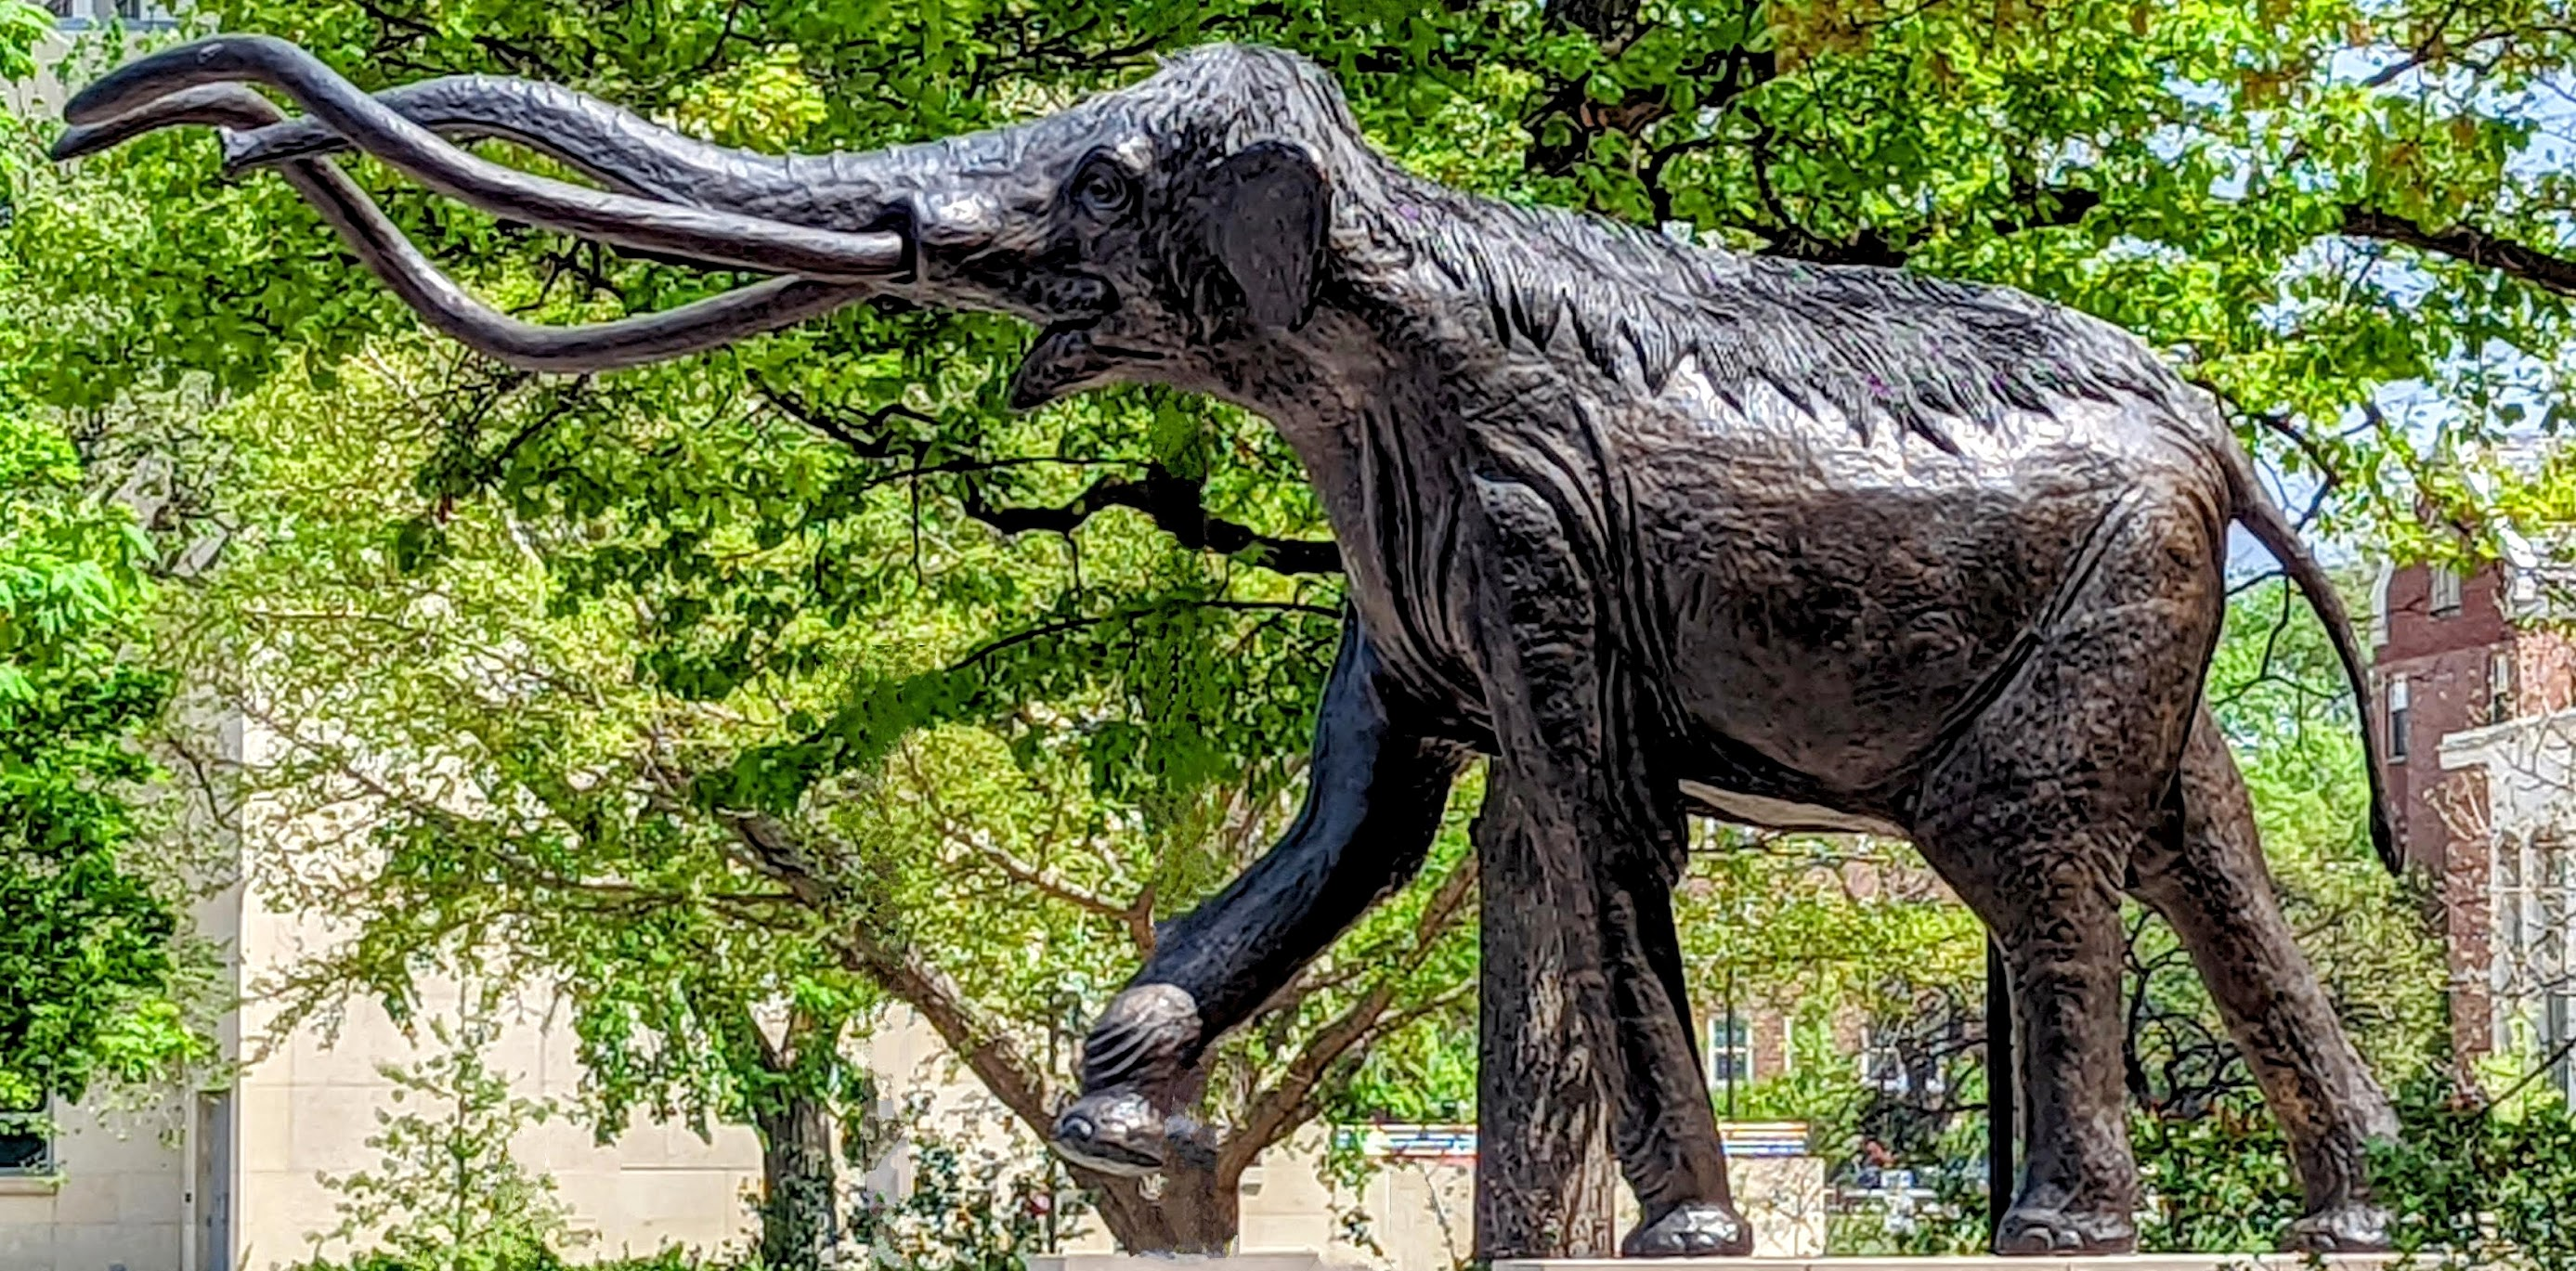
\includegraphics[width=.4\textwidth]{archie}
        \caption{Archie.\\ \footnotesize{Photograph by Bohn.}}
    \end{wrapfigure}

    You're relaxing at your favorite hangout when another customer catches your attention.
    He's rather large (dare I say, \textit{mammoth}), a bit hairy, and looking frustrated in front of his laptop.
    ``I'm Archie,'' he says, ``and I'm trying to teach myself this card game called \textit{Poker}.
    I found this source code that I thought I could use to understand Poker better, but the code is incomplete, and I don't entirely understand what's there.
    Could you explain the code to me, please?'
}

\newcommand{\GetHired}{
    Archie's face lights up in a very big smile.
    ``Thanks!''
    After pausing in thought for a moment, he says, ``Say, I've got a new startup company that could really use your help.
    Are you interested?
    It'll be exciting!''
}

\newcommand{\FirstDayOnTheJob}{
    \begin{wrapfigure}{r}{0.33\textwidth}
        \centering
        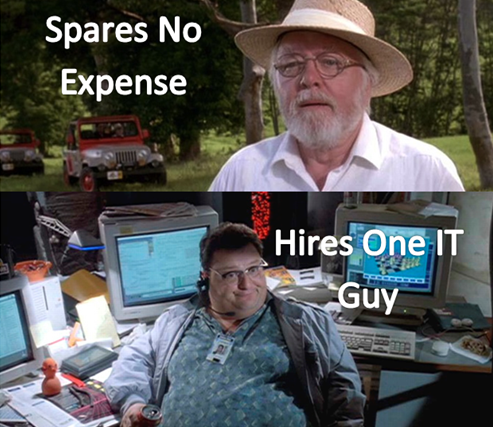
\includegraphics[width=.4\textwidth]{some-expenses-spared}
        \caption{Some expenses were spared.\\ \footnotesize{Original images \textcopyright\ Universal Studios and Amblin Entertainment, Inc. Meme creator unknown.}}
    \end{wrapfigure}

    You've recently been hired to help get the Pleistocene Petting Zoo get started.
    Your new employer, Archie, is surprisingly honest: he admits to you that some expenses were spared.
    Archie cheerfully points out that any challenge is also an opportunity to succeed.
    You suspect your job will offer plenty of ``opportunities to succeed.''
}

\newcommand{\HasKeyboard}{
    Great news!
    Archie brings you your new keyboard.
    He also brings you a problem of his own.
    Because you were held up with the broken keyboard, Archie decided to try some programming on his own, and his code is behaving strangely.
}

\newcommand{\ArchieWroteSmellyCode}{
    Working at the Pleistocene Petting Zoo certainly is proving to be interesting.
    You're glad that you don't have to worry about the problem of the giant sloths very slowly chasing their handlers, but now it seems that Archie has decided to try to write a program or two.
    At a glance, his code is smellier than the wooly rhinoceros' enclosure.
    But you take a closer look anyway to try to understand why his code acts strangely.
}

\newcommand{\InsurancePreview}{
    You hear somebody enter the room.
    ``\textit{Frankenstein}, `boat','' is the challenge, and she answers, ``borne.''
    Archie introduces you to the new arrival, ``Lil, this is our new developer, the one who wrote the app we just used.''
    He turns to you: ``This is Lilith Redd from business operations.''
    He turns back to her and continues, ``Lil, what's the good word?''

    ``The word isn't good, I'm afraid.
    I just heard back from the insurance company.''
}

\newcommand{\OnLoanToEclecticElectronics}{
    All work at the Pleistocene Petting Zoo has stopped while Archie tries to find a $\cancelto{\mathrm{reasonable}}{\mathrm{gullible}}$ insurance company.
    Rather than furloughing staff, he's asked everybody to help out with his other startup companies for a week or two.
    He specifically asked that you help out with Eclectic Electronics.

    Herb Bee, the chief engineer, explains that Eclectic Electronics is developing a patent-pending C-licon tool that will convert C code into an integrated circuit that has the same functionality as the original C code.
    To test it out, he tasked you with writing the code to implement an Arithmetic Logic Unit (ALU).
    Your task will be to implement integer addition, subtraction, multiplication, and division.
    Even though high-level languages' \textit{logical} boolean operations normally are not part of an ALU, Herb wants you to include these in the ALU to see if that can make some programs run faster.
    Because bitwise operations and bit shift operations have been implemented, you will be able to use C's bitwise and bit shift operators, but because arithmetic operations have not yet been implemented, you cannot use C's arithmetic operators.
    Because C library functions generally make use of arithmetic operations (which have not yet been implemented), you cannot use library functions.
}

\newcommand{\SuccessfulALU}{
    Herb smiles as he hands you the the test results from the latest integrated circuit fab batch.
    ``C-licon successfully turned your code into an ALU.
    Nicely done!''
    I think maybe it's time to use C-licon to see if we can improve the Floating Point Unit (FPU) on our experimental microprocessor.
}

\newcommand{\WriteAnFPU}{
    Herb tells you that, Eclectic Electronics tested the integrated circuit that the C-licon tool created from your ALU code, and they've concluded that C-licon is ready to use for their new experimental microprocessor.
    He tasks you with writing C code (that will be used by the C-licon tool) to implement a Floating Point Unit (FPU).
    Your task will be to implement floating point addition, subtraction, multiplication, and division.
    You can use any bit operations and, thanks to the ALU you wrote, you can use any integer arithmetic operations (use the conventional + - * / operators).
    Because the FPU has not yet been implemented, you cannot use C's floating point operations, you cannot use \lstinline{float}s nor \lstinline{double}s, and you cannot use library functions.
}

\newcommand{\GoingBackToTheZoo}{
    Lil enters the room.
    Herb challenges her: ``\textit{Gulliver's Travels}, `endian','' and Lil answers, ``ends.''

    Lil walks up to you and says, ``We have the insurance situation taken care of, and it's time to get the Zoo ready for guests.
    We're reassembling the tech team, and there's plenty of work to do.''

    You smile.
    ``That's good news!''

    Lil's face is hard to read.
    ``Well, yes and no.
    It's good that you'll be able to resume work on the Zoo's systems.
    But while Archie was waiting for us to fix the insurance situation, he got bored and -- cutting a long story short -- he ended up creating some new `opportunities' that we need you `to succeed' at.''
}

\newcommand{\SettledIntoRoutine}{
    You've settled into a comfortable routine at the Pleistocene Petting Zoo.
    While your job isn't quite as exciting as that of the saber-toothed tigers' dentist, it still has something new and interesting almost every day.

    Archie announces that he heard that hand-crafted assembly code can be faster than high-level language code.
    You try to explain that while this may have been true decades ago, modern optimizing compilers generate code faster than what a typical programmer can achieve with assembly code.
    Archie doesn't believe you and insists that you write the zoo's new cipher program in x86 assembly code.
}

\newcommand{\NewmanRanOffWithSamples}{
    Archie is hurriedly packing is trunk, like he's about to leave on a short-notice urgent trip.
    Before charging out the door, he pauses to tell you, ``Newman just stole some of our samples.
    I need to track him down before he sells them to the Supersized Safari Syndicate.
    I guess this means you're in charge of the Zoo's computer system now.
    Don't worry, you'll be fine. What could possibly go wrong?''
}

\newcommand{\BombLabIntroduction}{  % Ties Bryant & O'Halloran's Bomb Lab into the Pleistocene Petting Zoo story
    In a jarring collision of movie franchises, the CEO of Virtucon makes a Zoom call to the Pleistocene Petting Zoo.
    For some reason that nobody really explains, you're the only person available to handle the situation.
    The guy, who sounds kind of like an animated ogre, demands that the Pleistocene Petting Zoo deliver to him a megalodon shark with a head-mounted laser capable of emitting a beam of pure antimatter.

    You blurt out, ``Then it's not a laser,'' and then try to explain to him that megalodons are from the Miocene epoch, and expecting to find them at the Pleistocene Petting Zoo would be as ridiculous as a Cretaceous-period tyrannosaur at a Jurassic-themed park.

    ``Zip it!'' commands the guy who kind of looks like the host of a public-access show you used to watch.
    ``Since you won't meet my demand, my minions have placed a `binary bomb' under your zoo.
    Because I like really convoluted plans, we put software on your Linux server that controls the bomb.
    If you do nothing, the bomb will explode.
    If you turn off the Linux server, the bomb will explode.
    If you go slower than 50mph, the bomb will -- no, never mind that last part.

    ``The bomb software consists of a sequence of phases.
    Each phase expects you to type a particular string on \texttt{stdin}.
    If you type the correct string, then the phase is {\em defused} and the bomb proceeds to the next phase. Otherwise, the bomb {\em explodes}.
    The bomb is defused when every phase has been defused.

    ``Your mission, which you have no choice but to accept, is to defuse your bomb before the due date.
    Good luck, and welcome to the bomb squad!''
}

\newcommand{\FoodLockersAreStuck}{
    Having saved the Zoo from Dr. Evil's binary bomb, you relax back in your chair and think about taking a break.
%SPRINGBREAK
    Maybe an entire week in which you don't have solve any problems or meet any deadlines -- that'd be real nice.
%FALLBREAK
    % Maybe 4-day weekend in which you don't have solve any problems or meet any deadlines -- that'd be real nice.

    Another Zoom call comes in.
    \textit{What now!?} you wonder as you take your feet off of the desk to answer the call.
    An uncomfortable-looking animal handler says, ``We can't unlock the food lockers.
    It's the animals' feeding time, and we can't open the food lockers!
    It's feeding time, we can't get to the animals' food, and,'' his eyes dart nervously toward the animal enclosures, ``and many of them have sharp, pointy claws and others have big, stompy feet.''
}

\newcommand{\AttackLabIntroduction}{    % Ties Bryant & O'Halloran's Attack Lab into the Pleistocene Petting Zoo story
    You managed to keep the Pleistocene Petting Zoo from blowing to smithereens, but it turns out that Dr. Evil's minions weren't too careful when they put the bomb control software on the Zoo's Linux server.
    The software that controls the food locker has been heavily damaged!
    The functions that unlock the food locker doors are still present, but there's no way to activate those functions.

    You then recall what Archie told you when he hired you: some expenses were spared.
    You run the machine code through a disassembler and quickly see that it has a buffer overflow vulnerability.
    Before the situation in the dire wolf enclosure gets too dire, you sit down and get to work.

    The \function{ctarget} code runs on an older machine that allows executable code to be present on the stack, so it's vulnerable to a conventional code injection buffer overflow attack.
    \begin{itemize}
        \item Phase 1 (\function{touch1}) unlocks the food locker so the animal handlers can prepare the food.
        \item Phase 2 (\function{touch2}) opens the doors between the food locker and the carnivore enclosures;
        you will need to pass a cookie to the function to authenticate yourself.
        \item Phase 3 (\function{touch3}) closes the doors between the food locker and the carnivore enclosures.
    \end{itemize}
    The \function{rtarget} code runs on a newer machine that does not allow executable code to be present on the stack, so you'll have to conduct a return-oriented programming attack on it.
    \begin{itemize}
        \item Phase 4 (\function{touch2)} opens the doors between the food locker and the herbivore enclosures;
        you will need to pass a cookie to the function to authenticate yourself.
        \item Phase 5 (\function{touch3}) closes the doors between the food locker and the herbivore enclosures.
    \end{itemize}
}

\newcommand{\MostAnimalsAreFed}{
    Before you take on the Phase 5, pause to consider what you have accomplished so far.
    In Phases 2 and 3, you caused a program to execute machine code of your own design.
    If {\sc ctarget} had been a network server, you could have injected your own code into a distant machine.
    In Phase 4, you circumvented two of the main devices modern systems use to thwart buffer overflow attacks.
    Although you did not inject your own code, you were able inject a type of program that operates by stitching together sequences of existing code.
    Also, all animals have been fed, the carnivores are still in their enclosure, the mammoths can't fit through the herbivore door, and only the giant sloths seem interested in very slowly escaping.
}

\newcommand{\ArchieReturns}{
    Archie returns from tracking down Newman, who'd run off with some of the Pleistocene Petting Zoo's samples shortly before Dr.~Evil's Zoom call.
    ``It turns out he didn't get very far at all,'' Archie sighs.
    ``He ran into a flock of terror birds as he was leaving, and we found him in one of the emergency shelters.

    Archie smiles. ``I trust things were uneventful while I was away?''
}

\newcommand{\PickingUpNewmansProject}{
    Archie seems genuinely surprised that Newman is refusing to go back to work.
    ``You would think that he'd be grateful for being rescued from that flock of terror birds.''
    Before you can wonder out-loud whether it would be a good idea to trust someone who had just tried to sell trade secrets to a competitor, Archie gives you your new task.

    ``Because Newman isn't cooperating, I need you to finish the project he was working on.
    As you can imagine, duplicating the genetic information for our exhibits can take a long time, and Newman realized that we might be able to duplicate the data faster if we had a concurrent program which has one thread reading from the original data and another thread writing the copy.
    Unfortunately, he ran off to sell samples to the  Supersized Safari Syndicate before finishing the duplicator.
    Right now the duplicator seems to work, but it usually makes imperfect copies.
    Have you ever seen a paleolama with two noses, four eyes, and no ears!?''
}

\newcommand{\WeNeedBetterDetection}{
    Between Newman trying to sell samples to a competitor, that weird guy almost blowing up the zoo, and the animals almost escaping, Archie is getting worried.
    ``I think we need to introduce additional protective measures.
    As useful as your challenge-response app is in helping us detect intruders, I think it's now clear that we need something that will detect someone -- or some\textit{thing} -- when they're someplace they shouldn't be, even when no one else is around.
    I've asked the team at Eclectic Electronics to put something together.''
}

\newcommand{\WeNeedBetterLocks}{
    Between Newman trying to sell samples to a competitor, that weird guy almost blowing up the zoo, and the animals almost escaping, Archie is getting worried.
    ``I think we need to introduce additional protective measures.
    As useful as your challenge-response app is in helping us detect intruders, I think it's now clear that we need something that will keep someone -- or some\textit{thing} -- out of places they shouldn't be, even when no one else is around.
    I've asked the team at Eclectic Electronics to put something together.''
}

\newcommand{\IntroduceHardware}{
    Archie walks up to you, along with Herb Bee from Eclectic Electronics.
    Herb is holding a tangled mess of electronics.
    Archie explains, ``Herb here has developed a prototype of a device that he thinks will be useful for our physical security needs, as well as a few other applications around here. He calls it the \textit{Cow Pi}.''

% TODO: parameterize based on which microcontroller is actually being used
    You look at the device in Herb's hands and see the \nano\ central to the circuit.
    ``Isn't \textit{-Pi} typically used as a suffix for circuits that use a Raspberry Pi instead of an Arduino?''

    Herb replies, ``Typically, yes, but \textit{Cowduino} isn't very punny, is it?''

    Archie chimes in, ``Maybe with the right emphasis: \textit{Cow-DOO-ino}.''

    ``That's kind of subtle, don't you think? How will people know to put the emPHAsis on that sylLAble?''

    ``I think we're getting off topic here,'' you point out.
    ``How can I help?''

    ``Oh, right,'' Herb says, ``We'd like you to kick its proverbial tires.
    Let's start off with something simple, like a number builder tool.''
}

\newcommand{\JeffGoldblum}{
    Herb looks over your work.
    ``Hmm, yes. I think this is coming along nicely.
    Let's run a few more tests.''

    Archie storms into the room.
    ``We have \textit{got} to do something about security!
    How's that doodad coming along?
    Because there's now a half-man/half-fly in the labs going on-and-on about Chaos Theory and how if we just give him a MacBook and a spaceship then he'll be able to get the Lord of Thunder to travel across the 8th Dimension.
    Is that thing just about ready?''

    Herb shakes his head, ``No, not quite yet. It should be ready in about a week.''
}

\newcommand{\DisdainfulHerb}{
    Smoke wafts from Herb's soldering iron as he looks up when you approach.
    Cleaning the iron's tip, he quotes:
    ``Somebody once said, `The three most dangerous things in the world are a programmer with a soldering iron, a hardware engineer with a software patch, and'{}'' -- he glances nervously in Archie's direction -- ``{}`a user with an idea.'\footnote{
        Rick Cook, \textit{The Wizardry Consulted}, 1995.
    }$^{\mathrm{,}}$\footnote{
        The notion of being wary of programmers wielding screwdrivers or soldering irons long pre-dated this quote, as there are apocryphal tales of people who found it easier to modify the hardware to suit the software rather than the other way around.
    }''
}

\newcommand{\NumberConversionTool}{     % Since we're now allowing `sprintf()` with the LCD1602, converting between decimal and hexadecimal is trivial; it still might be okay for 7-segment displays
    Herb gets straight to the point.
    ``We promised Archie that we'd be able to start using the Cow Pi to build systems in a week.
    So far we've tested its input/output functionality, but we still need to test its timer and also whether we can take inputs without constantly polling the input devices.
    As before, we don't need to do anything too fancy;
    let's try a number base conversion tool.''
}

\newcommand{\LessDisdainfulHerb}{
    Smoke wafts from Herb's soldering iron as he looks up when you approach.
    Cleaning the iron's tip, he notes:
    ``Somebody once said that one of the most dangerous things in the world is a programmer with a soldering iron.''\footnote{
        ``The three most dangerous things in the world are a programmer with a soldering iron, a hardware engineer with a software patch, and a user with an idea.'' -- Rick Cook, \textit{The Wizardry Consulted}, 1995.
    }$^{\mathrm{,}}$\footnote{
        The notion of being wary of programmers wielding screwdrivers or soldering irons long pre-dated this quote, as there are apocryphal tales of people who found it easier to modify the hardware to suit the software rather than the other way around.
    }
}

\newcommand{\RemoteControlledCar}{

    About this time, Archie walks by, thinking about electric carts to transport visitors around the Pleistocene Petting Zoo.
    ``They probably should be remote-controlled.''
    He looks at you and Herb, and asks, ``Do you think you could make a cart a remote-controlled cart?''

    You ask the obvious question, ``Are there carts here already?''

    Archie waves his hand in the air, dismissing that detail, ``Not yet, but could you make the remote-control?''
    
    You hestatingly summarize: ``You want a cartless remote-controlled cart?''

    Archie beamingly smiles, ``Exactly!''

    Herb jumps in, ``Yes, we'll do it.''
    Herb looks at you and adds, ``It'll give us a chance to test the Cow Pi's timer and whether we can take inputs without constantly polling the input devices.''
}

\newcommand{\LauraDern}{
    You and Herb look for Archie in the Pleistocene Petting Zoo's labs to give him the good news, and you find a blond woman wearing cargo shorts, butchering a Gilbert and Sullivan song\dots \\ \\
    \textmusicalnote\ I am the very model of a modern vice admiral \textmusicalnote \\
    \textmusicalnote\ I've information about all things paleobotanical \textmusicalnote \\
    \textmusicalnote\ And I've been up to my armpits in problems scatological \textmusicalnote \\
    \textmusicalnote\ During the regency I had experience matriarchical \textmusicalnote \\
    \textmusicalnote\ I plot space travel, normal and superluminal \textmusicalnote \\
    \textmusicalnote\ (Even if I challenge the Pauli exclusion principle) \textmusicalnote \\

    ``I don't know how these people keep getting into our labs.
    \textit{Please} tell me that you have good news,'' pleads Archie.

    ``Yes, the Cow Pi is ready for whatever you need: calculators, security systems, parking meters -- you name it,'' Herb cheerfully responds.

    ``Excellent.''
    Archie turns to you.
    ``I'd like you and Newm... no, \textit{not} Newman.
    I'd like you and someone else on the staff to get started right away.
    Here's what I'd like to have built first.''
}

\newcommand{\CalculatorNeeded}{
    ``I have various teams working on different projects around here to improve security,'' Archie reminds you.
    He glances toward the Zoo's labs, where there's now a guy who looks like the actor who portrayed the fictional actor who portrayed the Norse god Odin, trying to avoid children while wistfully talking about raising rabbits in Montana.
    You briefly wonder why there are children someplace where there are also carnivorous megafauna, and then you remember that you work at a petting zoo.
    ``What I need your team to do,'' Archie continues, ``is make a four-function calculator so that we can quickly and easily determine whether we have the correct number of specimens, or if any are missing.''
}

\newcommand{\CalculatorCounting}{
    Technicians are using your calculator to compute how many specimens are still present in the lab, and establish that all specimens are accounted for after Newman's attempted theft.
    As reports come in of facilities getting secured with Cow Pi-based locks and passages being monitored with Cow Pi-based motion sensors, Archie smiles and tells you that this was a job well done.
    With all of the excitement neatly wrapped-up and arriving at a satisfactory conclusion, you look forward to a boring career in which there's absolutely no screaming and running for your life.
}

\newcommand{\CombinationLockNeeded}{
    ``I have various teams working on different projects around here to improve security,'' Archie reminds you.
    He glances toward the Zoo's labs, where there's now a guy who looks like the actor who portrayed the fictional actor who portrayed the Norse god Odin, trying to avoid children while wistfully talking about raising rabbits in Montana.
    You briefly wonder why there are children someplace where there are also carnivorous megafauna, and then you remember that you work at a petting zoo.
    ``What I need your team to do,'' Archie continues, ``is make a combination lock so that only authorized people can get into our lab facilities.''
}

\newcommand{\CombinationLockInstalled}{
    After fastening the new electronic combination lock to the lab door, Archie smiles and tells you that this was a job well done.
    With all of the excitement neatly wrapped-up and arriving at a satisfactory conclusion, you look forward to a boring career in which there's absolutely no screaming and running for your life.
}

\newcommand{\RangeFinderNeeded}{
    ``I have various teams working on different projects around here to improve security,'' Archie reminds you.
    He glances toward the Zoo's labs, where there's now a guy who looks like the actor who portrayed the fictional actor who portrayed the Norse god Odin, trying to avoid children while wistfully talking about raising rabbits in Montana.
    You briefly wonder why there are children someplace where there are also carnivorous megafauna, and then you remember that you work at a petting zoo.
    ``What I need your team to do,'' Archie continues, ``is make a range finder that will alert us when someone -- or some\textit{thing} -- gets too close to someplace they shouldn't be.''
}

\newcommand{\RangeFinderDetecting} {
    A technician installing a new range finder outside the lab door briefly sets off the alarm, but then the range finder falls quiet and faithfully reports that nothing is approaching.
    As reports come in of facilities getting secured with Cow Pi-based locks, and of accurate speciment counts accomplished with Cow Pi-based calculators, Archie smiles and tells you that this was a job well done.
    With all of the excitement neatly wrapped-up and arriving at a satisfactory conclusion, you look forward to a boring career in which there's absolutely no screaming and running for your life.
}

\usepackage{amsmath}
%\usepackage{array,color,colortbl}
\definecolor{LightGreen}{rgb}{0.88,1,0.88}
\usepackage{multicol}
\setlength{\columnsep}{2cm}
\usepackage{pdflscape}


% \captionsetup{width=.8\linewidth}

% \lstset{language=c, numbers=left, showstringspaces=false,
%     moredelim = [s][\ttfamily]{/*}{*/} % I shouldn't need this parameter!
%     }

\renewcommand{\labnumber}{\pollinglabnumber}
\renewcommand{\labname}{Using Polling with Memory-Mapped Input/Output}
\renewcommand{\shortlabname}{memory-mapped i/o -- pollinglab}
\renewcommand{\collaborationrules}{\pollinglabcollaboration}
\renewcommand{\duedate}{\pollinglabdue}
\newcommand{\nano}{\developmentboard} % TODO: replace \nano with \developmentboard
\renewcommand{\runtimeenvironment}{\pollinglabenvironment}
\pagelayout
\begin{document}
    \labidentifier

    \pdfbookmark[1]{Frontmatter}{frontmatter}                                       In this assignment, you will write code for \runtimeenvironment\ that will use new electronic devices to interact with the physical world.

The instructions are written assuming you will edit the code in the Arduino IDE and run it on \runtimeenvironment, constructed according to the pre-lab instructions.
If you wish, you may edit the code in a different environment; however, our ability to provide support for problems with other IDEs is limited.

\section*{Learning Objectives}

After successful completion of this assignment, students will be able to:
\begin{itemize}
    \item Work collaboratively on a hardware/software project
    \item Design and implement a simple embedded system
    \item Expand their programming knowledge by consulting documentation
\end{itemize}

\subsection*{Continuing Forward}

This penultimate lab assignment does not contribute to the final lab assignment.
By integrating elements of what you learned in this course, and by demonstrating that you can review documentation to learn on your own, to design a small embedded system, you will show how much progress you have made this semester.

\section*{During Lab Time}

During your lab period, coordinate with your group partner(s) to decide on your working arrangements.
Unless you're only going to work on the assignment when you're together, you may want to set up a private Git repository that is shared with your partner(s).
With your partner(s), modify your hardware kit as described in Section~\ref{sec:hardwareMods}.
Then, think through your system's design and begin implementing it.
The TAs will be available for questions.


    \softwareengineeringfrontmatter

    \section*{Scenario}                                                             \IntroduceHardware

    \section{Assignment Summary}                                                    This assignment is principally about getting comfortable when explicitly working with memory.
Being able to think about a value and a reference to that value distinctly will improve your programming skills in any language.

Before you do so, in Section~\ref{sec:archiesCode} you will examine Archie's code.
Parts of Archie's programs use code that the C standard explicitly states will result in undefined behavior.
By understanding the mistakes that Archie made, we hope that you can avoid them in your own code.

In Section~\ref{sec:challengeResponse}, you will build and use a linked list.
This will require you to allocate space for the list's nodes and manipulate pointers that connect the nodes to each other.

\ifboolexpe{not bool{allowspaghetticode}}{
    There are no particular restrictions in this assignment other than those common to most lab assignments in this course.
    You can check whether you're using a \lstinline{goto} or \lstinline{continue} statement, or whether you're using \lstinline{break} or \lstinline{return} to exit a loop, by running the constraint-checking Python script:
    \texttt{python constraint-check.py linkedlistlab.json}
}{}


    \section{Getting Started} \label{sec:GettingStarted}                            Download \textit{\shortlabname.zip} or \textit{\shortlabname.tar} from \filesource\ and copy it to \runtimeenvironment.
Once copied, unpackage the file.
Four of the five files (\textit{alu.h}, \textit{basetwo.c}, \textit{alu.c}, and \textit{integerlab.c}) contain the starter code for this assignment.
The last file (\textit{Makefile}) tells the \texttt{make} utility how to compile the code.
To compile the program, type:

\texttt{make}

This will produce an executable file called \textit{integerlab}.

When you run the program with the command \texttt{\textbf{\textit{./integerlab}}}, you will be prompted:

\begin{verbatim}
    Enter a one- or two-operand logical expression,
        a two-operand comparison expression, a two-operand arithmetic expression,
        "lg <value>" or "exponentiate <value>" to test your powers-of-two code,
        "is_negative <value>" to determine if 2's complement value is negative,
        "add1 <binary_value1> <binary_value2> <carry_in>" for 1-bit full adder,
        "add32 <hex_value1> <hex_value2> <carry_in>" for 32-bit ripple-carry adder,
        or "quit":
\end{verbatim}

When you enter a value, if it is prepended with \texttt{\textbf{\textit{0x}}} then the parser will parse it as a hexadecimal value;
otherwise, except as noted in Sections~\ref{subsec:one-bit-full-adder} and \ref{subsec:ripple-carry-adder}, the parser will treat it as a decimal value.

For now, type \texttt{\textbf{\textit{quit}}} to exit the program.

\subsection{Description of IntegerLab Files}

\subsubsection{integerlab.c}

Do not edit \textit{integerlab.c}.

This file contains the driver code for the lab.
It parses your input, calls the appropriate arithmetic function, and displays the output.

\subsubsection{alu.h} \label{subsubsec:alu.h}

Do not edit \textit{alu.h}.

This header file contains two type definitions:
\begin{description}
    \item[one\_bit\_adder\_t] is a structure to hold the 1-bin inputs (\lstinline{a}, \lstinline{b}, \lstinline{c_in}) and 1-bit outputs (\lstinline{sum}, \lstinline{c_out}) of a one-bit full adder.
    \item[alu\_result\_t] is a structure to hold the outputs from an arithmetic logic unit.
        Its fields are:
        \begin{itemize}
            \item \lstinline{result}, a 16-bit bit vector that is considered ``the'' result of the computation
            \item \lstinline{supplemental_result}, a 16-bit bit vector that stores additional result data from instructions that place their results in two registers
            \item \lstinline{unsigned_overflow}, a 1-bit flag to indicate whether overflow occurred when interpreting the source operands as unsigned values
            \item \lstinline{signed_overflow}, a 1-bit flag to indicate whether overflow occurred when interpreting the source operands as signed values
            \item \lstinline{divide_by_zero}, a 1-bit flag to indicate whether there was an attempt to divide by zero.
        \end{itemize}
\end{description}

The header file also contains two macros, \function{is_zero()} and \function{is_not_zero()} to bootstrap your ALU code.
These macros act like functions and return a boolean value to indicate whether an integer is 0 or not.\footnote{
    The astute student will quickly realize that \function{is_not_zero()} is not necessary and, with a little thought, will realize that they can \function{is_zero()} as a function within the constraints of this assignment.}

The header file also contains several function declarations.
The requirements for these functions will be discussed later in this assignment.

\subsubsection{basetwo.c}

This is the first of two files that you will edit.

There are two functions in \textit{basetwo.c} that will allow you to demonstrate an understanding of powers-of-two and/or an understanding of some uses of bit shifts.
\begin{description}
    \item[lg()] returns the base-2 logarithm of its argument, assuming its argument is a positive power-of-two;
        if the argument is 0 or is not a power-of-two, then there are no guarantees about the function's return value
    \item[exponentiate()] creates a power-of-two by raising 2 to the provided exponent, assuming the exponent is a non-negative value strictly less than 32;
        if the argument is negative or is greater than 31, then there are no guarantees about the function's return value
\end{description}
These functions are inverses of each other: $x = \log_2 2^x$, and $y = 2^{\log_2 y}$.

Strictly speaking, you can write your ALU code without these functions;
however, some students in the past had difficulty finding solutions for their ALU code without obtaining a base-2 logarithm and/or calling a function to create a power-of-two.
Rather than tempt you to violate one of the assignment's constraints by calling the \textit{math} library's \function{log2()}, \function{exp2()}, and/or \function{pow()} functions, we now have you write your own code for these functions.

\subsubsection{alu.c}

This file will contain most of the code that you write, and the functions in \textit{alu.c} are in the order in which you will likely write them.
\begin{itemize}
    \item A simple check
        \begin{description}
            \item[is\_negative()] returns a boolean value to indicate whether the argument, when interpreted as a signed integer, is negative
        \end{description}
    \item Equality comparisons
        \begin{description}
            \item[equal()] returns \lstinline{true} if and only if $value1 = value2$
            \item[not\_equal()] returns \lstinline{true} if and only if $value1 \not = value2$
        \end{description}
    \item Logical operations
        \begin{description}
            \item[logical\_not()] returns the logical inverse of the argument
            \item[logical\_and()] returns the logical conjunction of the two arguments
            \item[logical\_or()] returns the logical disjunction of the two arguments
        \end{description}
    \item Addition and subtraction
        \begin{description}
            \item[one\_bit\_full\_addition()] performs addition for one bit position, determining both the sum bit and the carry-out bit
            \item[ripple\_carry\_addition()] adds two 32-bit values to each other and to a carry-in bit
            \item[add()] adds two 16-bit values to each other
            \item[subtract()] subtracts a 16-bit value from another
        \end{description}
    \item Inequality comparisons
        \begin{description}
            \item[less\_than()] returns \lstinline{true} if and only if $value1 < value2$
            \item[at\_most()] returns \lstinline{true} if and only if $value1 \leq value2$
            \item[at\_least()] returns \lstinline{true} if and only if $value1 \geq value2$
            \item[greater\_than()] returns \lstinline{true} if and only if $value1 > value2$
        \end{description}
    \item Unsigned multiplication and division
        \begin{description}
            \item[multiply\_by\_power\_of\_two()] multiplies the first argument by the second, assuming that the second argument is zero or a power of two;
                there are no guarantees if this assumption is not satisfied
            \item[unsigned\_multiply()] multiplies two 16-bit values to each other, if the arguments are interpreted as unsigned integers
            \item[unsigned\_divide()] divides a 16-bit value by another, if the arguments are interpreted as unsigned integers
        \end{description}
    \item Signed multiplication and division (bonus credit)
    \begin{description}
        \item[signed\_multiply()] multiplies two 16-bit values to each other, if the arguments are interpreted as signed integers
        \item[signed\_divide()] divides a 16-bit value by another, if the arguments are interpreted as signed integers
    \end{description}
\end{itemize}


    \section{Initial Changes to the Code} \label{sec:LabTime}                       During your lab period, the TAs will guide the class through the first modifications to the starter code that you must make, described in this section.
If you do not attend your lab period, then you must complete this section on your own.
\textbf{\textit{Except during lab time, you may }not\textit{ discuss the solutions for this section with other students.}}


\subsection{Reviewing the Datasheet}

Read the Datasheet sections that discuss \href{https://cow-pi.readthedocs.io/en/latest/microcontroller.html#interrupts}{Interrupts} and \href{https://cow-pi.readthedocs.io/en/latest/microcontroller.html#timers}{Timers}.

You can skip over the section that covers registering external interrupt handlers using \function{attachInterrupt()}, as we will use pin change interrupts.
You can skip over the section that covers the timers ``Normal'' mode, as we will use ``Clear Timer on Compare'' (CTC) mode.
You can skip over the section that covers configuring TIMER0, as we will use only TIMER1 and TIMER2.

\subsection{Examining the Starter Code}

Familiarize yourself with the functions in \textit{character\_selector} and \textit{message\_editor} and the header comments that describe what the functions will do.

\subsection{Debouncing} \label{subsec:debouncing}

When you place your code that responds to key presses and button presses in the interrupt handlers, place it inside the braces for the \function{debounce_interrupt()} macro.
Just as the \function{cowpi_debounce_byte()} function took care of debouncing when polling mechanical inputs, the \function{debounce_interrupt()} macro defined in \textit{inputs.h} takes care of (most of) the debouncing when mechanical inputs generate interrupts.
There are two catches.

The first catch is that \function{debounce_interrupt()} only works when the interrupt handler responds to both the rising and falling edges of the input.
This isn't such a terrible limitation, as a pin change interrupt is fired whenever there is a change on a pin.
That is, your ISR will be invoked whenever there is a key/button press \textit{or} release --
so you already have to be able to handle both presses and releases.
If the interrupt is due to a press, then take the appropriate actions;
if the interrupt is due to a release, then do nothing.

The second catch is that \function{debounce_interrupt()} works by ignoring interrupts that are generated due to switchbounce.
It does not -- it cannot -- ignore switchbounce that occurs while the interrupt handler is executing.
Consider this scenario: the user presses a button, closing the contacts, triggering an interrupt, and the interrupt handler launches.
Before reaching the code that reads the inputs to determine which key was pressed (or whether a button was pressed or released), the switch bounces, temporarily re-opening the contacts;
when the code reads the inputs, the wrong condition is detected!
The fix is to introduce a loop that iterates until a sensible input reading is found.
This busy-wait loop is already in the starter code.


\subsection{Handling Key Presses}

\subsubsection{The Interrupt Service Routine}

In \textit{inputs.c}, locate the \function{initialize_interrupts()} function.
In this function:
\begin{itemize}
    \item Use \function{cowpi_register_pin_ISR()} to register \function{handle_keypress()} as the interrupt service routine that should be invoked whenever there is key movement on the keypad.
\end{itemize}

\paragraph{Hint} Which microcontroller pins did you use to detect key movement in PollingLab? \\

Locate the \function{handle_keypress()} function.

After the busy-wait loop terminates, the \lstinline{key} variable holds the character corresponding to the key that was pressed, or \lstinline{'\0'} if no key was pressed (\textit{i.e.}, a key was released).
\begin{itemize}
    \item Add code that will call the \function{update_character()} function if a key was pressed.
\end{itemize}

\subsubsection{The Logic} \label{subsubsec:logic}

In \textit{character\_selector.c}, locate the \lstinline{characters} and \lstinline{key_modulus} arrays.
The \lstinline{characters} nested array describes the characters that can be produced by cycling through each of the numeric keys on the keypad.\footnote{
    A ``box'' character is used in place of a space character so that it's more clear on the display module whether a blank at the end of the message is meant to be a space or is merely an empty blank.
}
The \lstinline{key_modules} array describes how many useful characters are in each of \lstinline{characters}' rows.\footnote{
    Because \lstinline{characters} is a nested array, all rows occupy 5 bytes, even though most rows don't have five useful characters.
}

The \lstinline{working_key} global variable selects the \lstinline{characters} row, and the \lstinline{character_index} global variable selects the column.
The \function{reset_selector()} function sets both of these variables to -1, using named constants to provide meaning to these special values.

Locate the \function{update_character()} function in \textit{character\_selector.c}.
In this function:
\begin{itemize}
    \item Determine if the input is valid.
    \item If so, determine what the first character should be, according to Requirements~\ref{spec:keypad} and \ref{spec:firstPress},
        and send that character to the message editor using the \function{replace_character()} function.
\end{itemize}
(The \function{update_character()} function will have more responsibility later,
but for now, just focus on sending a character to the message editor.)

In \textit{message\_editor.c}, locate the \lstinline{message} array and related variables.
The \lstinline{message} array is a buffer to store the message being edited,
and \lstinline{message_index} is used to track the end of the message.
The \lstinline{display_start} pointer is used to indicate the start of the substring that will be displayed on the display module.

Locate the \function{replace_character()} function in \textit{message\_editor.c}.
In this function:
\begin{itemize}
    \item Add code to place the character in the \lstinline{message} buffer at \lstinline{message_index}.
        Do \textit{not} update \lstinline{message_index}.
\end{itemize}
(You will make further changes to the \function{replace_character()} function later,
but for now, just focus placing the character at the end of the string.)

\subsubsection{Test Your Code}

At this point, all characters are placed at the start of the message, but you can still check:
\begin{itemize}
%    \item Does your code cycle through the characters for each key?
    \item Does your code produce the first character from each number key's character sequence?
    \item Does your code produce characters for all the number keys?
    \item Does your code produce characters for only the number keys?
\end{itemize}


\subsection{Blinking the LED} \label{subsec:blinking}

According to Requirement~\ref{spec:pressIndicator}, the right LED needs to blink for approximately \textonequarter second whenever the user presses a key.

In \textit{inputs.c}, locate the \lstinline{led_timer} pointer and the \lstinline{supplemental_counter} variable.
The \lstinline{led_timer} pointer is a pointer to a structure for an 8-bit timer;
we will have it point to the memory-mapped I/O registers for TIMER2.
Unfortunately, the greatest interrupt period possible for TIMER2 is 16.384ms, well short of \textonequarter second.
Our solution to this is to use \lstinline{supplemental_counter} to count the number of times that TIMER2 fires an interrupt,
and take further action only when \lstinline{supplemental_counter}'s value indicates that approximately \textonequarter second has passed.

\subsubsection{Configuring the Timer}

We will approximate \textonequarter second as 256ms.
The reason for this is that we want our ISRs to execute as fast as possible, and if we tried to take action after exactly 250ms, we will have to resort to division, which takes hundreds of cycles on the ATmega328P microcontroller.
If we choose to take action after 256ms, then we can select a power-of-two, $n$ such that the ISR takes action once every $n$ times that the ISR runs.
Now, we can determine when the ISR has run $ISR$ times by adding 1 to \lstinline{supplemental_counter} each time the ISR runs and then applying a bitmask ($n-1$).
This effectively will cause overflow every 16, 32, 64, 128, or 256 increments.
Now, the desired interrupt period is $\frac{256}{n}ms$.

In \function{initialize_interrupts()}:
\begin{itemize}
    \item Consulting the Datasheet's \href{https://cow-pi.readthedocs.io/en/latest/microcontroller.html#configuring-timer2}{Configuring TIMER2} section.
        Assign the base address for TIMER2's registers to \lstinline{led_timer}.
    \item Using the equation in the Datasheet's \href{https://cow-pi.readthedocs.io/en/latest/microcontroller.html#clear-timer-on-compare-mode}{Clear Timer on Compare Mode} section,
        select a prescaler such that the resulting comparison value is at most $2^8$.
    \item Using the Datasheet's Tables 17--19, construct a bit vector for TIMER2's control register for ``CTC'' mode with your chosen prescaler.
        Assign this bit vector to \lstinline{led_timer}'s \lstinline{control} field.
    \item Subtract 1 from your calculated comparison value, and assign the result to \lstinline{led_timer}'s \lstinline{compareA} field. \\
        \textcolor{red}{IMPORTANT! The assignment to the \lstinline{compareA} field must occur \textit{after} the assignment to the \lstinline{control} register.}
    \item Consulting the Datasheet's \href{https://cow-pi.readthedocs.io/en/latest/microcontroller.html#timer-interrupts}{Timer Interrupts} section, enable the \lstinline{TIMER2_COMPA_vect} interrupt vector by setting the \lstinline{OCIE2A} bit to 1.
\end{itemize}

In \function{reset_timers()}:

\begin{itemize}
    \item Uncomment \lstinline{led_timer->counter = 0;}
\end{itemize}

\subsubsection{Turning the LED On and Off}

According to Requirement~\ref{spec:pressIndicator}, the right LED shall illuminate when the user presses a key.
\begin{itemize}
    \item Add a call to \function{cowpi_illuminate_right_led()} in the part of \lstinline{inputs.c} that will run when a key has been pressed.
    \item Immediately after that, reset the timers' counters and the supplemental counter to zero.
\end{itemize}

According to Requirement~\ref{spec:pressIndicator}, the right LED needs to deluminate after approximately \textonequarter second, which we are approximating as 256ms.
Locate the code in \textit{inputs.c} that looks like this:

\begin{lstlisting}
    ISR(TIMER2_COMPA_vect) {
        ;
    }
\end{lstlisting}

\begin{itemize}
    \item Add code to that block to increment \lstinline{supplemental_counter} and to cause it to overflow after the requisite number of increments.
    \item Add code to that block that will call \function{cowpi_deluminate_right_led()} whenever \lstinline{supplemental_counter} overflows.
\end{itemize}

You should take the time to convince yourself that the LED will turn off exactly 256ms after a key is pressed.
You should take the time to convince yourself that there will be no observable effect when \lstinline{supplemental_counter} overflows while the LED is off.


\subsubsection{Test Your Code}

The easy part of testing this code is: when you press a key, does the right LED turn on and then off again?

Testing that the LED illuminates for exactly 256ms is a bit harder to do on a human scale, but you can give yourself a sanity check.
Briefly practice pressing a key repeatedly, and try to get the cadence of pressing a key such that it re-illuminates almost the instant that it starts to dim.
Have a friend or lab partner open the stopwatch app on their smartphone.
Have them give you a ``ready, set, go!'' lead-in, and then call time five seconds later.
When your friend or lab partner tells you to go, start pressing a key with that cadence -- \textbf{\textit{count the number of presses until they call time}}.
If you counted 18 or 19 key presses, then your illumination time is in the right ballpark.

\vspace{1cm}

You are now ready to complete the remainder of this assignment on your own.
Reminders:
\begin{itemize}
    \item You can complete Sections~\ref{sec:characterGeneration} and \ref{sec:oddsAndEnds}.
    \item \collaborationrules
\end{itemize}



    \section{Memory-Mapped Input/Output} \label{sec:MemMapIO}                       In this section, you will use the data structures provided by the CowPi library to access the \processor's memory-mapped I/O registers.
All functions that you edit in this part of the assignment are in \textit{io\_functions.c}
You will use the same test code from Section~\ref{sec:LabTime} to test your code.

\textit{Remember that to start the I/O test code, the \textbf{left switch} must be in the \underline{right} position when the Cow~Pi restarts.}

You can complete this part of the assignment before or after implementing the system from Section~\ref{sec:SimpleSystem}.
You must, however, complete Section~\ref{sec:LabTime} first.
If you have already implemented the system from Section~\ref{sec:SimpleSystem}, you may want to make a backup copy of your program now.


\subsection{Reading a Timer} \label{subsec:timer}

Because you have already completed Section~\ref{sec:LabTime}, you can use the \lstinline{timer} pointer to access the
\ifdefstring{\processor}{ATmega328P}{\lstinline{cowpi_timer8bit_t}}{}
\ifdefstring{\processor}{RP2040}{\lstinline{cowpi_timer_t}}{}
structure, which overlays the \processor's
\ifdefstring{\processor}{ATmega328P}{TIMER0.}{}
\ifdefstring{\processor}{RP2040}{general-purpose timer.}{}
Use the
\ifdefstring{\processor}{ATmega328P}{\lstinline{counter}}{}
\ifdefstring{\processor}{RP2040}{\lstinline{raw_lower_word}}{}
field to access the
\ifdefstring{\processor}{RP2040}{lower 32~bits of the}{}
timer's value.
No debouncing code is necessary because, while the timer's value can be thought of as an input, it is not a mechanical switch.

Locate the \function{get_microseconds()} function.
In the starter code, this function is implemented by calling the Arduino \function{micros()} function to report the time elapsed, in microseconds, since the microcontroller was powered-up.

\ifdefstring{\processor}{ATmega328P}{
    The \processor's TIMER0 is configured to increment its value every 4 microseconds.
    Because the timer's value is an 8-bit value, it overflows every $256 \times 4 = 1024$ microseconds.
    The starter code tracks how many times the timer overflows and stores that value in the \lstinline{timer_overflow_count} global variable.
    The total time since the sytem was powered up can be determined by finding out how much time had elapsed at the last overflow and how much time has elapsed since the last overflow.
    \begin{description}
        \checkoffitem{Replace the call to \function{micros()} with code that:}
        \begin{description}
            \checkoffitem{Multiplies \lstinline{timer_overflow_count} by 1024. This is how much time had elapsed at the last overflow.}
            \checkoffitem{Uses the \lstinline{timer} pointer to read from the timer's \lstinline{counter} field and multiply that value by 4. This is how much time has elapsed since the last overflow.}
            \checkoffitem{Returns the sum of those two products.}
        \end{description}
    \end{description}
}{}
\ifdefstring{\processor}{RP2040}{
    The \processor's timer value increments every microsecond.
    \begin{description}
        \checkoffitem{Replace the call to \function{micros()} with code that uses the \lstinline{timer} pointer to obtain the timer's value.}
        \begin{description}
            \checkoffitem{Read from the timer's \lstinline{raw_lower_word} field and return that value.}
        \end{description}
    \end{description}
}{}

\subsubsection*{Test your code}

\begin{description}
    \checkoffitem{Place the both switches in the \textit{right} position and upload your code.}
\end{description}
The output will show the elapsed time, a small fraction of a second.
Whenever you press/release a key, press/release a button, or toggle a switch, the display will update the elapsed time.
\begin{description}
    \checkoffitem{Open your smartphone's clock app, and go to the stopwatch feature.}
    \checkoffitem{Press the Cow~Pi's RESET button and the stopwatch's START button at the same time.}
    \checkoffitem{Press a button on the Cow~Pi a few times, comparing the elapsed time on the stopwatch and the elapsed time on the Cow~Pi's display.}
\end{description}


\subsection{Simple Inputs and Outputs} \label{subsec:simpleIO}

Because you have already completed Section~\ref{sec:LabTime}, you can use the
\ifdefstring{\processor}{ATmega328P}{\lstinline{ioports} pointer as an array of \lstinline{cowpi_ioport_t} structures, which you can index using the \lstinline{D0_D7}, \lstinline{D8_D13}, and \lstinline{D14_D19} named constants.}{}
\ifdefstring{\processor}{RP2040}{\lstinline{ioport} pointer to access the \lstinline{cowpi_ioport_t} structure that overlays the data pins' registers.}{}
Use the \lstinline{.input} field with bitmasks to read inputs.
Use the \lstinline{.output} field with bitmasks and the read-modify-write pattern to write outputs.
During lab, the TAs covered reading from inputs and using the read-modify-write pattern to write outputs;
however, if you missed lab or have forgotten, you can find examples in the section of the Cow~Pi datasheet that \href{https://cow-pi.readthedocs.io/en/latest/CowPi_\lowercaseprocessor/io_registers.html#structure-for-memory-mapped-input-output}{discusses the \lstinline{cowpi_ioport_t} structure}.

\subsubsection{Simple Inputs}

Locate the \function{left_button_is_pressed()}, \function{right_button_is_pressed()}, \\ \function{left_switch_in_right_position()}, and  \function{right_switch_in_right_position()} functions.
In the starter code, these functions are implemented by calling functions in the CowPi library.

\begin{description}
    \checkoffitem{Replace the calls to CowPi library functions with code that uses the \lstinline{ioports} array to ascertain the controls' positions. \\
        \textcolor{red}{Do \textit{not} remove the calls to \function{debounce_byte()}!}}
\end{description}

\paragraph{Test your code}

\begin{description}
    \checkoffitem{Place the \textbf{left switch} in the \textit{right} position and the \textbf{right switch} in the \textit{left} position, and upload the program to your Cow~Pi.}
\end{description}
The output will include the positions of the left and right buttons (``U'' for up and ``D'' for down) and of the left and right switches (``L'' for left position and ``R'' for right position).


\subsubsection{Simple Outputs}

Locate the \function{set_right_led()} function.
In the starter code, this function is implemented by calling functions in the CowPi library.

\begin{description}
    \checkoffitem{Modify this function to replace the calls to CowPi library functions with code that uses the \lstinline{ioports} array to turn the LED on or off.}
    \begin{description}
        \checkoffitem{Use the read-modify-write pattern to do so, so that you do not change any pins that you do not intend to change.}
        \item[\phantom{xxx}$\bullet$] No debouncing code is necessary because these functions do not read from mechanical switches.
    \end{description}
\end{description}

\paragraph{Test your code}

\begin{description}
    \checkoffitem{Place the \textbf{left switch} in the \textit{right position} and upload the program to your Cow~Pi.}
\end{description}
If both switches are in the right position then the right LED will illuminate.

\vspace{1cm}

This would be a good time to make a backup copy of your program.


\subsection{Scanned Input} \label{subsec:ScannedInput}

Now that you have some practice with using memory-mapped I/O to read from and write to external pins, you can demonstrate your understanding by combining reads and writes to deduce which key (if any) on the keypad is being pressed.

Locate the \function{get_keypress()} function.
The implementation in the starter code calls the CowPi library's \function{cowpi_get_keypress()} function.
The \function{cowpi_get_keypress()} function returns a \lstinline{char} corresponding to the character on the pressed key,
but the \function{get_keypress()} function is supposed to return a \lstinline{uint8_t} that has the hexadecimal value of the pressed key (considering \# as 0xE and * as 0xF).
Because of this, the rest of the implementation is a pair of \lstinline{switch} statements to obtain the correct value from the \function{keys} nested array.

Read the section of the Cow Pi datasheet that \href{https://cow-pi.readthedocs.io/en/latest/hardware/inputs.html#matrix-keypad}{discusses the matrix keypad}.
After you have done so:

\begin{description}
    \checkoffitem{Preserve the debouncing code in \function{get_keypress()}, and}
    \checkoffitem{Replace the starter code's call to \function{cowpi_get_keypress()} and its \lstinline{switch} statements with code that scans the keyboard.}
        \begin{description}
            \checkoffitem{Use the \lstinline{ioports} array to read from and write to the appropriate pins,}
            \checkoffitem{Use a $1\mu s$ busy-wait (see below) for the delay shown on line 4 of the pseudocode in the datasheet, and}
            \checkoffitem{Use the \lstinline{keys} nested array to obtain the correct integer value for the key at a given row and column.}
        \end{description}
\end{description}

\paragraph{What is a busy-wait?}
A busy-wait is a loop that does nothing until some criterion is satisfied.
\begin{lstlisting}[numbers=none, basicstyle=\ttfamily\small]
    while (!condition_is_satisfied) {}
\end{lstlisting}
In this case, the condition to be satisfied as that at least one microsecond has elapsed since the busy-wait started.
\begin{description}
    \checkoffitem{Use \function{get_microseconds()} to obtain the time immediately before the busy-wait.}
    \checkoffitem{In the busy-wait, compare that with the ``current'' value obtained by \function{get_micrseconds()} to see if at least one microsecond has elapsed.}
\end{description}

\subsubsection*{Suggestions}
Look at the pseudocode\footnote{
    Note that the pseudocode uses the ``walrus operator'' (\texttt{:=}) for assignments and the ``equal sign'' (\texttt{=}) for equality comparisons, as is common in ALGOL-inspired languages.
    This is in contrast to C-inspired languages that use the ``equal sign'' for assignment and the ``double equal sign'' for equality comparisons.
} in the datasheet and relate it to the ``theory of operation.''
Even though the pseudocode is expressed as nested loops, you do not need to implement it that way.
We have seen implementations that have an outer loop for the rows and an inner loop for the columns,
and we have seen implementations that have a loop for the rows but use a \lstinline{switch} statement or chained \lstinline{if} statements to enumerate the possibilities for the columns.
With four rows and four columns, both are viable solutions.

The key insights are:
\begin{itemize}
    \item Each of the row vectors you output will have exactly one ``0'' bit;
        the placement of that ``0'' corresponds to exactly one of the rows in the \lstinline{keys} nested array, and
    \item Each of the column vectors you read as input, if it is not 0xF, will have exactly one ``0'' bit;
        the placement of that ``0'' corresponds to exactly one of the columns in the \lstinline{keys} nested array
\end{itemize}

Even though you \textit{can} set the loop conditions to terminate the loop as soon as the pressed key has been determined,\footnote{
    I am \textit{not} saying you can \lstinline{return} from inside the loop or \lstinline{break} out of the loop;
    I am saying you can write a \lstinline{while} condition that includes testing whether \lstinline{key_pressed} is still 0xFF.
} it would be better to keep your loop conditions simple and allow the code to examine all sixteen keys.
With only sixteen keys, there isn't much time savings to be had by ending the loop as soon as the key has been found,
and in a ``real'' embedded system, our time budget would have to allow enough time to examine all sixteen keys and so any ``savings'' gained by ending the loop early would be lost to sitting idle later.

\subsubsection*{Test your code}

\begin{description}
    \checkoffitem{Place the \textbf{left switch} in the \textit{right} position and the \textbf{right switch} in the \textit{left} position, and upload the program to your Cow~Pi.}
\end{description}
The output will include the key that was pressed (if any), a hyphen if no key is being pressed, or a question mark if \function{get_keypress()} returns an invalid value.

\vspace{1cm}

This would be a good time to make a backup copy of your program.


%\subsection{Display Module} \label{subsec:DisplayModule}
%
%You will use a pointer to a \lstinline{cowpi_i2c_t} structure to access the memory-mapped I/O registers for the \processor's I$^2$C (aka ``TWI'') hardware,
%and you will use those registers to send data to the display module.
%
%Read the datasheet's sections that discuss
%the \href{https://cow-pi.readthedocs.io/en/latest/microcontroller.html#atmega328ptwistruct}{I$^2$C registers},
%the \href{https://cow-pi.readthedocs.io/en/latest/microcontroller.html#controller-transmitter-sequence}{I$^2$C Controller Transmitter Sequence},
%the \href{https://cow-pi.readthedocs.io/en/latest/hardware/outputs.html#data-byte-for-lcd1602-display-module}{data format for bytes sent to the display module},
%and the \href{https://cow-pi.readthedocs.io/en/latest/hardware/outputs.html#hd44780-driven-lcd-character-display}{steps required by the display module itself}.
%After you have done so, review the starter code for
%
%\begin{lstlisting}[numberstyle=\color{gray}, numbers=left, firstnumber=285, basicstyle=\ttfamily\small, escapechar=`]
%    void send_halfbyte(const cowpi_display_module_protocol_t *configuration, uint8_t halfbyte, bool is_command) {
%        // contact the peripheral by transmitting a start bit followed by the desired peripheral's address
%        cowpi_i2c_initialize(configuration);    `\label{code:i2cInitialize}`
%        // (you do not need to make further use of the `configuration` argument)
%
%        // transmit one or more data bytes
%        // (your code goes here)                `\label{code:i2cData}`
%
%        // transmit a stop bit
%        cowpi_i2c_finalize();                   `\label{code:i2cFinalize}`
%    }
%\end{lstlisting}
%
%Of the \href{https://cow-pi.readthedocs.io/en/latest/microcontroller.html#controller-transmitter-sequence}{three steps} in the I$^2$C Controller Transmitter Sequence, the first step of contacting the display module is handled in line~\ref{code:i2cInitialize},
%and the third step of transmitting a STOP bit is handled in line~\ref{code:i2cFinalize}.
%Your task is to implement the second step of transmitting one or more data bytes, starting at line line~\ref{code:i2cData}.
%These are \href{https://cow-pi.readthedocs.io/en/latest/hardware/outputs.html#hd44780-driven-lcd-character-display}{the bytes and the requisite delay} required by the display module.
%
%If you have not already done so:
%
%\begin{itemize}
%    \item Uncomment the second line of the starter code's \function{initialize_io()} function, and
%    \item Assign the appropriate address to the \lstinline{i2c} pointer on that line.
%\end{itemize}
%
%Then, starting at line line~\ref{code:i2cData}:
%
%\begin{itemize}
%    \item Implement the pseudocode from the I$^2$C Controller Transmitter Sequence's ``transmit one or more data bytes'' step, to
%    \item Send the three bytes of data required by the display module.
%        \begin{itemize}
%            % \item You may handle the error conditions show in the pseudocode in whatever manner you see fit; it would be best to do so in a manner that allows you to determine \textit{which} error is occurring.
%            \item Use \lstinline{delayMicroseconds(1)} to implement the pulse described in the \href{https://cow-pi.readthedocs.io/en/latest/hardware/outputs.html#data-byte-sequence}{data byte sequence}.
%        \end{itemize}
%\end{itemize}
%
%After you are satisfied that you have implemented the \function{send_halfbyte()} function correctly:
%
%\begin{itemize}
%    \item Uncomment the last line of the starter code's \function{initialize_io()} function to register \function{send_halfbyte()} with the CowPi\_stdio library.
%\end{itemize}
%
%All of the functions in the CowPi library that send characters or commands to the display module will now make use of your \function{send_halfbyte()} function.
%
%\subsubsection*{Suggestions}
%Altogether, your code will make three transmissions in the \function{send_halfbyte()} function.
%After each transmission, you need to wait until the transmission is complete before initiating the next transmission;
%you can achieve this with a \textit{busy wait}.
%As discussed in lecture, a busy wait is simply a do-nothing loop that blocks the program while some condition holds.
%
%The bit vector created in line~6 of the the Controller Transmitter Sequence's pseudocode consists of bits that must be set to 1 in the control register for all of these transmissions.
%
%Even though the pseudocode might appear to characterize those transmissions as a loop over the data meant for the display module, the \texttt{for each} statement should be understood to mean $\forall$ -- indeed, it will be easier to implement the byte sequence sequentially.
%Two of the three bytes meant for the display module are identical, and the remaining byte differs only only in one bit.
%The first ensures the halfbyte, backlight, read/write, and command bits are at their correct values before a latching pulse starts.
%The second maintains those values and creates the latching pulse; a \function{delayMicroseconds()} call holds the pulse.
%Finally, the third byte ensures those values are still present as the latching pulse ends.
%
%\vspace{0.5cm}
%
%There are two aspects to this task that some students found frustrating in the past:
%\begin{itemize}
%    \item Some of the required bitshifts may seem like make-work -- for example, line~16 of the pseudocode shifts the serial adapter's address to the left by one bit, but after that the least significant bit is always 0
%        \begin{itemize}
%            \item These bits that are seemingly constant appear so only because this assignment uses one specific part of a very flexible protocol
%            \item In other uses of the I$^2$C protocol, the bits that are constant \textit{in this assignment} serve other purposes
%        \end{itemize}
%    \item If some part of your implementation has a bug, you aren't provided with much data you can use to form hypotheses during debugging
%        \begin{itemize}
%            \item ``Not much data'' is not the same as ``no data''
%                \begin{itemize}
%                    \item If a busy-wait doesn't terminate, the problem is probably with your implementation of the I$^2$C protocol -- double-check the bit vectors placed in the control register%, and possibly the bit vector placed in the data register when you transmit the serial adapter's address
%                    \item If the function terminates but the display module doesn't update, the problem is probably with the bit vectors placed in the data register that the serial adapter will pass along to the display module, or with the ``latch'' pulse
%                \end{itemize}
%            \item You can always get help from the professor or a TA with any aspect of this assignment, and you can discuss \textit{concepts and syntax} with other students.
%                \textit{Without showing other students your code}, asking other students questions like these, and answering them, is acceptable:
%                \begin{itemize}
%                    \item ``The datasheet says we want a `1' in bit 7, a `1' in bit 2, and `0's in the other bits; that looks like this, right?'' and then write a binary or hexadecimal bit vector on paper or a whiteboard
%                    \item ``The datasheet says to shift a `1' seven places to the left, and then shift a `1' two places to the left, and then take those two results and bitwise-OR them together; would you help me remember how to do a left-shift?''
%                \end{itemize}
%        \end{itemize}
%\end{itemize}
%
%\subsubsection*{Test your code}
%
%Place the left switch in the right position and upload the program to your Cow~Pi.
%If the test code displays its outputs on the display module, then you implemented \function{send_halfbyte()} correctly.
%If the test code does not display its output one the display module, or if the test code does not run at all, then there is an error in your code.
%
%\vspace{1cm}
%
%If you decide to work on other parts of the assignment before finishing \function{send_halfbyte()} then comment-out the assignment to \lstinline{cowpi_hd44780_send_halfbyte} in \function{initialize_io()}.


    \section {Implementing a Simple System Using Polling} \label{sec:SimpleSystem}  In this section you will implement a ``number builing tool'' that turns a sequence of inputs into a number.
A notional use of this number builder would be to create the operands for a calculator.
Section~\ref{sec:FunctionalSpecification} has the tool's specification.
You should design your system using the I/O functions -- either the implementations from the starter code with the debouncing code added, or the implementations you wrote (or will write) from Section~\ref{sec:MemMapIO}.
After the specification are a few suggestions for making good use of those functions.

If you have already implemented the I/O code from Section~\ref{sec:MemMapIO}, you may want to make a backup copy of your program now.

Make sure that \textit{number\_builder.ino}'s \function{loop()} function calls \function{build_number()} and not \function{test_io()}.


\subsection{Number Builder Specification} \label{sec:FunctionalSpecification}

\begin{enumerate}
\item The tool shall have two alignment modes, \textit{left justified mode} and
    \textit{right justified mode}. The \textbf{left switch} controls the alignment mode.
    When the \textbf{left switch} is toggled to the left, the tool shall be in left justified mode.
    When the \textbf{left switch} is toggled to the right, the tool shall be in right justified mode.
\item The tool shall have two number bases, \textit{decimal} and
    \textit{hexadecimal}. The \textbf{right switch} controls the number base.
\item \label{spec:decimalExplained} When the \textbf{right switch} is toggled
    to the left, the number builder will use the decimal number base. When the
    user presses a button on the \textbf{matrix keypad} with a decimal numeral
    (\textit{0-9}) then the number builder shall take the appropriate action as
    specified in requirement \ref{spec:initialKeyPress} or
    \ref{spec:BuildingValue}. Any other buttons on the keypad shall be ignored.
\item \label{spec:hexadecimalExplained} When the \textbf{right switch} is
    toggled to the right, the number builder will use the hexadecimal number
    base. When the user presses a button on the \textbf{matrix keypad} then the
    number builder shall take the appropriate action as specified in
    requirement \ref{spec:initialKeyPress} or \ref{spec:BuildingValue}.
    Buttons with decimal numerals (\textit{0-9}) or alphabetic letters
    (\textit{A-D}) shall be interpreted as having the corresponding hexadecimal
    numeral; the button with the octothorp (\#) shall be interpreted as having
    the hexadecimal numeral \textit{E}; and the button with the asterisk (*)
    shall be interpreted as having the hexadecimal numeral \textit{F}.
\item Initially, the \textbf{display module} shall be blank.
\item \label{spec:illuminateLED} Whenever the user presses a key on the
    \textbf{matrix keypad}, the \textbf{right LED} (aka, the external LED) shall
    illuminate for approximately one-half of a second. Whenever the user presses
    one of the \textbf{pushbuttons}, the \textbf{left LED} (aka the internal LED)
    shall illuminate for approximately one-half of a second.
\item The \textbf{LEDs} shall not illuminate except as specified in
    requirement~\ref{spec:illuminateLED}.
    %Exception: the \textbf{left LED} may blink as a consequence of its pin being used as the SPI \texttt{SCK} signal.
    There is no prohibition against the \developmentboard's \texttt{TX},
    \texttt{RX}, and \texttt{PWR} LEDs illuminating.
\item The system shall build numbers in response to user input:
    \begin{enumerate}
    \item The numbers' values shall be representable as 32-bit signed integers.
    \item \label{spec:initialKeyPress} If the display is blank
        (\textit{i.e.}, there is not yet a number being built), then whenever the
        user presses a button on the \textbf{matrix keypad}, the corresponding
        numeral shall be displayed on the \textbf{display module}'s top row,
        either in the far-left column or the far-right column, depending on the
        alignment mode. The numeral displayed shall follow the interpretations
        specified in requirements \ref{spec:decimalExplained} and
        \ref{spec:hexadecimalExplained}.
    \item \label{spec:BuildingValue} If the display is not blank (\textit{i.e.},
        there is a number being built), then whenever the user presses a button
        on the \textbf{matrix keypad}, the corresponding numeral shall become
        the least-significant digit of the number shown on the
        \textbf{display module}; all pre-existing digits shall increase in
        significance by one order of magnitude. For example, if \display{234} is
        displayed and the user presses \texttt{5}, then \display{2345} shall be
        displayed. The numeral displayed shall follow the interpretations
        specified in requirements \ref{spec:decimalExplained} and
        \ref{spec:hexadecimalExplained}.
        \begin{enumerate}
        \item There shall be no noticeable lag in updating the display.
        \item The alignment mode shall be preserved. If in left justified mode,
            then the most-significant digit shall remain in the leftmost column.
            If in right justified mode, then the new least-significant digit
            shall be in the rightmost column.
        % \item \label{spec:printValueToConsole} The new value shall be printed
        %     to the Serial Monitor in decimal or hexadecimal, depending on the
        %     system's current number base.
        \end{enumerate}
    \item ``0x'' shall be displayed as part of a hexadecimal value.
    % \item ``0x'' shall not be displayed as part of a hexadecimal value.
    \item Whenever the user presses the \textbf{left pushbutton}, the value
        being displayed shall be negated.
        \begin{enumerate}
        \item In the decimal number base, the presence or absence of negative
            sign shall indicate whether or not a value is negative.
        \item In the hexadecimal number base, 32-bit two's complement shall be
            used.
        \end{enumerate}
    \item A positive sign shall not be displayed as part of a positive value.
    \item If a negative decimal value is displayed, the negative sign shall
        be displayed immediately to the left of the most-significant digit
        being displayed. For example, \display{-456} is correctly
        displayed, but \display{-\phantom{xxxx}456} is not correctly displayed.
        \begin{enumerate}
        \item If in left justified mode, the negative sign shall be in the
            leftmost column, and the most-significant digit shall be in the
            column immediately to the right of that.
        \end{enumerate}
    \item Leading 0s may be displayed but are discouraged. For example,
        \display{782} is preferred, but \display{00000782} is allowed.
    \item Digit separators are permitted but not required. For example, both
        \display{12345} and \display{12,345} are acceptable, as are both
        \display{0x6789A} and \display{0x6,789A}.
    \item Whenever the user presses the \textbf{right pushbutton} while a number
        is being built, the number that has been built shall be displayed on the
        bottom row, aligned according to the alignment mode, for approximately
        one second. After approximately one second, the number that has been
        built shall reset to 0, and the \textbf{display module} shall be cleared.
        % \item In no case shall the tool allow the user to input a value too
        %     great to be displayed on the \textbf{display module}. If
        %     the user attempts to enter a value greater than $0x7FFF,FFFF$ in
        %     hexadecimal, less than $0x8000,0000$ in hexadecimal, greater than
        %     $99,999,999$ in decimal, or less than $-9,999,999$ in decimal, then the
        %     \textbf{display module} shall display \display{too big}.
        \item In no case shall the tool allow the user to input a value too
            great to be stored as a 32-bit signed integer. If the user attempts to
            enter a value greater than $0x7FFF,FFFF$ in hexadecimal, less than
            $0x8000,0000$ in hexadecimal, greater than $2,147,483,647$ in decimal, or
            less than $-2,147,483,648$ in decimal, then the \textbf{display module}
            shall display \display{too big}.
            \begin{itemize}
            \item \textit{n.b.}, in a hexadecimal 32-bit negative integer, an
                \texttt{F} in the most-significant hex-digit might only be a sign
                extension; in this scenario, if the user inputs another hex-digit
                then it is still a valid number because it would not be less than
                $0x8000,0000$. \\ \\
                For example, adding another digit to the 32-bit integer
                $0xF865,4321$ would \textit{not} produce a too-great value because
                the 36-bit integer $0xF,8654,3210 = -2,041,302,512_{10}$, and the
                32-bit integer $0x8654,3210 = -2,041,302,512_{10}$. Because
                $0x8000,0000 = -2,147,483,648_{10} \leq -2,041,302,512_{10}$, adding
                the \texttt{0} digit did not produce a ``too big'' value. \\ \\
                On the other hand, adding another digit to the 32-bit integer
                $0xF765,4321$ \textit{would} produce a too-great value because the
                36-bit integer $0xF,7654,3210 = -2,309,737,968_{10}$, but the 32-bit
                integer $0x8654,3210 = 1,985,229,328_{10}$. Because
                $0x8000,0000 = -2,147,483,648_{10} > -2,309,737,968_{10}$, adding
                the \texttt{0} digit did produce a ``too big'' value.
            \end{itemize}
    \end{enumerate}
\item If the user toggles the \textbf{left switch} (\textit{i.e.}, changes
    alignment mode): if no number is being displayed, then the system shall
    seamlessly transition between alignment modes; otherwise, the system's
    behavior is undefined.
\item If the user toggles the \textbf{right switch} (\textit{i.e.}, changes
    the number base): if no number is displayed, or if the number 0 is displayed,
    then the system shall seamlessly transition between number bases; if a
    non-zero number is being built then the system's behavior is undefined.
\item \label{spec:singleKeypress} When the user presses a button for less than
    approximately one-half of a second, regardless of whether it is one of the
    \textbf{pushbuttons} or a key on the \textbf{matrix keypad}, it shall be treated
    as a single press.
\end{enumerate}


\subsection{Using I/O Functions}

The header comments for the I/O functions in the starter code amply describe the functions.
Updating the LEDs and reading the switches' positions require no special handling;
however, polling the momentary pushbuttons and the keypad keys requires some extra care.

\subsection{Implementing Requirement~\ref{spec:singleKeypress}}

When using interrupts to detect button presses or key presses, debouncing is sufficient to ensure that only one press is detected for each actual press.
When polling the momentary pushbuttons or keypad keys, each time the \function{loop()} function executes, their position will be queried.
The problem is that the control loop iterates much faster than a human can remove their finger, and so a single press of a button or key is detected many, many times.

You can overcome this problem by keeping track of the last time that each pushbutton was pressed and the last time that a keypress was detected.
Then add a guard to prevent polling a pushbutton or the keypad during the half-second after the last detection.
The code would look something like this:

\begin{lstlisting}
    if ((now - last_keypress > BUTTON_NO_REPEAT_TIME) &&
        (...)) {
      last_keypress = now;
      uint8_t keypress = get_keypress();
      ...
    }
\end{lstlisting}


\subsection{Detecting a Keypress}

Detecting presses of pushbuttons and determining which button was pressed are the same action: you know whether the right or left button was pressed by whether you detected the button press with \function{left_button_is_pressed()} or \function{right_button_is_pressed()}.
Because you don't want to unnecessarily scan the keypad, you should only call \function{get_keypress()} \textit{after} determining that a key pas been pressed.

As described in Section~1.2.1 of the Cow Pi datasheet, you can determine whether or not a key was pressed by examining the input pins connected to the keypad's columns (Arduino pins D14--D17).
If the values on all of these pins are 1, then no key is being pressed;
on the other hand, if one of the pins has the value 0, then a key is being pressed.
Once you have determined that a key is being pressed, you can call \function{get_keypress()}, knowing that it will return the value corresponding to one of the keys.


\subsection{Outputting to the Display Module}

You will not call \function{send_halfbyte()} directly.
Instead, you will call one or more of the CowPi library's functions that work with the LCD1602 display module; these functions, in turn, will make use of \function{send_halfbyte()} after you have implemented and registered it.
The functions are described in Section~2.5 of the Cow Pi datasheet.

You will want to read Section~1.3 of the Cow Pi datasheet to understand the addresses used by the \function{cowpi_lcd1602_place_character()} and \function{cowpi_lcd1602_place_cursor()}.
While the datasheet's Section~1.3 also describes shifting the display, there is no part of this lab assignment that calls for shifting the display.

    \section{Turn-in and Grading}                                                   \filesubmission.

\policyforcodethatdoesnotcompile

\latepolicy

\subsection*{Rubric}

This assignment is worth 35 points.
\begin{description}
    \rubricitem{1}{\function{is_nan()} correctly reports whether or not its argument is a number}
    \rubricitem{1}{\function{is_zero()} correctly reports whether or not its argument is zero}
    \rubricitem{1}{\function{is_infinity()} correctly reports whether or not its argument is infinite}
    \rubricitem{1}{\function{is_negative()} correctly reports whether or not its argument is negative}
    \rubricitem{1}{\function{get_754_integer()} correctly extracts the significand's implicit integer}
    \rubricitem{1}{\function{get_754_fraction()} correctly extracts the significand's fraction bits}
    \rubricitem{1}{\function{get_754_exponent()} correctly extracts the exponent}
    \rubricitem{1}{\function{decode()} correctly converts an \lstinline{ieee754_t} value into a \lstinline{unnormal_t} structure}
    \rubricitem{1}{\function{negate()} correctly changes its argument's sign}
    \rubricitem{5}{\function{add()} can add integers \& fractions, positive \& negative values, and ``large'' \& ``small'' numbers}
    \rubricitem{1}{The identity and commutative properties hold for \function{add()}}
    \rubricitem{1}{\function{add()} provides correct answers for its special cases}
    \rubricitem{5}{\function{multiply()} can multiply integers \& fractions, positive \& negative values, and ``large'' \& ``small'' numbers}
    \rubricitem{2}{The identity, zero, and commutative properties hold for \function{multiply()}}
    \rubricitem{1}{\function{multiply()} provides correct answers for its special cases}
    \rubricitem{1}{\function{divide()} provides correct answers for its special cases}
    \rubricitem{1}{\function{divide()} can divide when the divisor is of the form $\pm 2^n, -126 \le n \le 127$}
    \rubricitem{1}{\function{divide()} can divide when the dividend's significand is a multiple of the divisor's significand}
    \rubricitem{1}{\function{add()} demonstrates that \function{encode()} rounds down when the truncated part of the significand is less than halfway between representable values}
    \rubricitem{1}{\function{add()} demonstrates that \function{encode()} rounds up when the truncated part of the significand is more than halfway between representable values}
    \rubricitem{2}{\function{add()} demonstrates that \function{encode()} rounds to the nearest-even when the truncated part of the significand is exactly halfway between representable values}
    \rubricitem{1}{Rounding can carry into the exponent}
    \rubricitem{1}{\function{add()} and/or \function{multiply()} demonstrate that \function{encode()} overflows to infinity}
    \rubricitem{1}{\function{add()}, \function{multiply()}, and/or \function{divide()} demonstrate that \function{encode()} gracefully underflows through subnormal numbers}
    \rubricitem{1}{\function{multiply()} and/or \function{divide()} demonstrate that \function{encode() underflows to zero}}
    \bonusitem{2}{\function{divide()} can divide arbitrary values}
\end{description}

\textbf{Penalties}
\begin{description}
    \softwareengineeringpenalties
    \item[no credit] for functions that use \lstinline{float} or \lstinline{double} variables or constants, use \lstinline{union} variables, use C's floating point operations, and/or a function you did not write
    \item[no credit] for arithmetic functions, if \function{decode()} and/or \function{encode()}  use \lstinline{float} or \lstinline{double} variables or constants, use \lstinline{union} variables, use C's floating point operations, and/or a function you did not write
\end{description}


    \section*{Epilogue}                                                             \JeffGoldblum

    \textit{To be continued...}

    \newpage\appendix
%    \appendix

    \section{Appendix: Lab Checkoff}                                                You are not required to have your assignment checked-off by a TA or the professor.
If you do not do so, then we will perform a functional check ourselves.
In the interest of making grading go faster, we are offering a small bonus to get your assignment checked-off at the start of your scheduled lab time immediately after it is due.
Because checking off all students during lab would take up most of the lab time, we are offering a slightly larger bonus if you complete your assignment early and get it checked-off by a TA or the professor during office hours.

\begin{enumerate}
    \precheckoffitem{Position the Cow Pi a little more than 1~meter from a wall, or position an upright book (or other object) a little more than 1~meter from the Cow Pi.}
    \precheckoffitem{Place both switches in the left position.}
    \precheckoffitem{Upload your code to your \developmentboard, and leave your code open in the IDE.}
    \precheckoffitem{Confirm that the system detects the wall (or book or other object) and not something closer (such as a computer or the table surface).}

    \checkoffitem{Show and explain to the TA how your code generates a tone with a frequency of 5kHz; that is, it has a period of 200\textmu s.}
    \checkoffitem{Place the right switch in the right position, putting the system in Continuous Tone mode.
        The system generates a continuous 5kHz tone.}
    \item[] (TA, confirm that the tone is 5kHz by code inspection and by ear; confirm with the HuskerScope spectrum analyzer if you aren't sure.) \\
        \textit{+1 There is code to generate an audible tone} \\
        \textit{+1 The system continuously generates the tone when in Continuous Tone mode} \\
        \textit{+2 The audible tone has a frequency of 5kHz}

    \checkoffitem{Place the left switch in the right position, putting the system in Threshold Adjustment mode.
        The system prompts for a new threshold range. \\
        \textit{+1 The user is prompted to enter a new threshold range when the system is in Threshold Adjustment mode}}
    \checkoffitem{Enter a range of 25, using the `\#' key to indidicate that you have fininished entering the value.
        The system displays a helpful error message explaining that this is not a valid threshold range.
        The system then prompts the user for a new threshold range. \\
        \textit{+1 The user is given a helpful error message after entering an invalid threshold range} \\
        \textit{+1 The user is re-prompted to enter a threshold range after entering an invalid threshold range}}
    \checkoffitem{Enter a range of 450, using the `\#' key to indidicate that you have fininished entering the value.
        The system displays a helpful error message explaining that this is not a valid threshold range.
        The system then prompts the user for a new threshold range.}
    \checkoffitem{Enter a range of 75, using the `\#' key to indidicate that you have fininished entering the value.
        The system displays a message confirming the new threshold range. \\
        \textit{+2 Valid threshold ranges are those between 50cm and 400cm, inclusive} \\
        \textit{+1 The user is shown a confirmation message after entering a valid threshold range} \\
        \textit{+2 The user can enter a new threshold range when the system is in Threshold Adjustment mode}}

    \checkoffitem{Place the right switch in the left position, putting the system in Single Pulse mode.
        The system might indicate that no object has been detected yet; however, this is not required information before initiating a ping.}
    \checkoffitem{Show and explain to the TA how your code initiates a pulse.}
    \checkoffitem{Show and explain to the TA how your code measures the length of a pulse.}
    \checkoffitem{Show and explain to the TA how your code achieves the required precision (no greater than 1\textmu s) and accuracy (immediately detect pulse edges without waiting for code in the main loop to poll the pin).}
    \checkoffitem{Press the pushbutton to initiate a pulse.
        The right LED strobes once.
        The piezodisc does not chirp.
        The system displays the correct distance to the wall (or book or other object). \\
        \textit{+2 There is code to initiate an ultrasound pulse} \\
        \textit{+3 There is code to detect the length of the pulse} \\
        \textit{+3 The pulse's length is measured to a precision of no greater than 1\textmu s} \\
        \textit{+3 The pulse's length is measured as accurately as possible} \\
        \textit{+2 The user can request a ping when the system is in Single Pulse mode} \\
        \textit{+2 The distance to an object is correctly calculated from the pulse's length} \\
        \textit{+2 When an object is detected, the system displays the distance to the object} \\
        \textit{+2 When an object is detected in Single-Pulse mode, the system generates exactly one alarm} \\
        \textit{+2 A strobe is an illumination of the right LED for 50ms} \\
        \textit{+2 A strobe occurs for any detected object}}
    \checkoffitem{Slightly change the distance between the Cow Pi and the target object.
        Press the pushbutton to initiate a pulse.
        The LED strobes once.
        The piezodisc does not chirp.
        The system displays the new distance to the wall (or book or other object). \\
        \textit{+2 The user can request another ping when the system is in Single Pulse mode}}

    \checkoffitem{Place the left switch in the left position, putting the system in Normal Operation mode.
        The system displays the distance to the target object, and it displays an approach rate of 0cm/s.
        The LED strobes once per seccond (100ms), but the piezodisc does not chirp. \\
        \textit{+1 The switches control the mode of operation as specified} \\
        \textit{+2 When an object is detected in Normal Operation mode, the system repeatedly generates alarms}}
    \checkoffitem{Slowly move the Cow Pi closer to the wall, or slowly move the book (or other object) closer to the Cow Pi.
        As you do so, vary the rate of approach slighly to demonstrate that the rate of approach updates.
        The displayed distance changes with the decreasing distance to the target object.
        The system displays a plausible, positive rate of approach that updates at least once every second. \\
        \textit{+2 When an object is detected in Normal Operation mode the rate of approach is displayed} \\
        \textit{+2 When an object is detected in Normal Operation mode, the rate of approach is updated at least once every second}}
    \checkoffitem{As the distance between the Cow Pi and the target object decreases, note that:
        \begin{description}
            \item[When the distance falls below 100cm] the LED strobes more frequently, once every 750ms (\textthreequarters sec)
            \item[When the distance falls below 75cm] the piezodisc chirps every 750ms
            \item[When the distance falls below 50cm] the LED strobes, and the piezodisc chirps, every 500ms (\textonehalf sec)
            \item[When the distance falls below 25cm] the LED strobes, and the piezodisc chirps, every 250ms (\textonequarter sec)
            \item[When the distance falls below 10cm] the LED strobes, and the piezodisc chirps, every 125ms ($\frac{1}{8}$ sec)
        \end{description}
        \textit{+2 A chirp is an audible tone lasting 50ms} \\
        \textit{+2 When the system repeatedly generates alarms, the time between alarms is as specified}}

    \checkoffitem{Place the both switches in the right position, putting the system in Threshold Adjustment mode.
        The system prompts for a new threshold range.}
    \checkoffitem{Enter a range of 55.
        The system displays a message confirming the new threshold range.}
    \checkoffitem{Place the both switches in the left position, putting the system in Normal Operation mode.
        The system displays the distance to the target object, and it displays an approach rate of 0cm/s.}
    \checkoffitem{Slowly move the Cow Pi away from the wall, or slowly move the book (or other object) away from the Cow Pi.
        The displayed distance changes with the decreasing distance to the target object.
        The system displays a plausible, negative rate of approach.}
    \checkoffitem{As the distance between the Cow Pi and the target object decreases, the alarms become less urgent.
        Note that as the distance increases above 55cm, the piezodisc stops chirping but the LED continues to strobe. \\
        \textit{+2 A chirp occurs for a detected object that is closer than the threshold range} \\
        \textit{+2 A chirp only occurs for a detected object that is closer than the threshold range}}

    \checkoffitem{Reorient the Cow Pi, or remove the book (or other object) so that there are no in-range objects to detect.
        The system displays a message indicating that no object is detected.
        The LED does not strobe, and the piezodisc does not chirp.\\
        \textit{+3 The code correctly recognizes the that no object has been detected, if no object reflects the ultrasound pulse} \\
        \textit{+2 When there is no in-range object, the system displays a message to that effect} \\
        \textit{+2 A strobe only occurs for a detected object}}

    \checkoffitem{Show the TA any code they have not yet examined. \\
        \textit{+1 The code is clean, well-organized, has good variable and function names, and is otherwise understandable}}
\end{enumerate}

%    \newpage

    \section{Appendix: C Syntax Notes}                                              In this assignment, you will see some syntax that you haven't encountered before,
and you will see some syntax that you've seen but  may have not given much thought to.

\subsection{Variable Modifiers}

C has some keywords that can be used to modify variables.
In some cases, these keywords define scoping rules;
in other cases, these keywords provide information to the compiler that it can use when optimizing the resulting assembly code.

\subsubsection{const}

In LinkedListLab, you encountered the \lstinline{const} keyword.
When used as part of an ordinary variable declaration, it prevents the variable from being modified after it has been initialized.
(Much to some peoples' surprise, this does not actually make it a constant as far as C's syntax rules are concerned.)

When used with a pointer, the \lstinline{const} keyword tells the compiler that it can make optimizations under the assumption that whatever the pointer points to will not change.
Code that breaks this promise will have compile-time warnings, but it will compile and run -- but it often will have runtime errors.
(There is another way to use \lstinline{const} with a pointer that declares the pointer itself to be unchanging.)

\subsubsection{volatile}

In DuplicatorLab, you encountered the \lstinline{volatile} keyword.
A \lstinline{volatile} variable is the opposite of a \lstinline{const} variable:
not only can it change, it can spontaneously change.
The \lstinline{volatile} keyword tells the compiler that it cannot optimize-away a variable that is never written to.
It also tells the compiler that it cannot optimize-away a variable that is never read.

With threaded code such as what you saw in DuplicatorLab, it's tempting to believe that a sufficiently thorough static analysis of the code will reveal that a variable is being written to and/or read from multiple threads.
When working with memory-mapped input/output registers in this lab, you will read from variables that do not have a single line of code \textit{anywhere} changing their values, and yet their values will change.
Similarly, you will write to variables that do not have a single line of code anywhere that reads from them, and yet it is important that those variables be updated.

\subsubsection{extern}

You will typically see externalized variables in header files, and you can see one in \textit{io\_functions.h}.
The when a variable is declared with the \lstinline{extern} modifier, it does not define a new variable.
Instead, it allows functions in one \texttt{.c} file to access global variables that are defined in another \texttt{.c} file.
That is, it makes a global variable even more global.

\subsubsection{static}

The other modifier you will see in this lab is the \lstinline{static} keyword.
If you've programmed in Java, beware that C's \lstinline{static} keyword is not the same as Java's \lstinline{static} keyword.\footnote{
    Nor can it be.
    Java's \lstinline{static} keyword declares a field to belong to the whole class;
    C does not have classes.
}

\paragraph{Static global variables}

When used with a global variable, the \lstinline{static} keyword limits that variable's scope to code to the \texttt{.c} file it's defined in (or to the \texttt{.c} file that \lstinline{#include}s the \texttt{.h} file it's defined in).
This allows other code in \textit{other} files to have static global variables with the same name without a naming collision.
That is, it makes a global variable a little less global.

Similarly, the \lstinline{static} keyword can limit a function's scope.

\paragraph{Static local variables}

When used with a scope-limited variable, such as a variable declared in a function, the variable becomes something of a hybrid variable.
Unlike a normal function-local variable, which is allocated on the program stack, these \lstinline{static} variables are allocated on the heap.
When a function returns, normal function-local variables are deallocated because the function's stack frame is popped.
A \lstinline{static} variable, however, is \textit{not} deallocated when its function returns.
That means that its last value is still available the next time that the function is called.
A \lstinline{static} variable used in this way looks like a global variable -- its value is preserved between function calls -- but it is still scope-limited to the function it's declared in.

You can see examples of \lstinline{static} variables in the I/O test code.

You should explicitly initialize a \lstinline{static} variable on the same line that it is declared.
Such an initializer must be a syntactic constant.
The variable will only be initialized once; it will \textit{not} be reinitialized each time the function is called.
(If it were reinitialized, that would rather defeat the point of the variable preserving its value between function calls, right?)
If you do not explicitly initialize the variable then, unlike ordinary function-local variables, a \lstinline{static} variable will automatically be initialized to 0.

If you have questions about \lstinline{static} variables, please ask the professor or a TA\@.
You are not \textit{required} to use \lstinline{static} variables, but it is a good idea to do so because the alternative is introducing more global variables than you might otherwise need.

%\paragraph{Static array sizes}
%
%The other use of the \lstinline{static} keyword can be seen in the first parameter for \function{display_string()} function in \textit{supplement.h}.
%\begin{lstlisting}
%    static inline void display_string(
%        const char string[static (NUMBER_OF_DISPLAYABLE_COLUMNS+1)],
%        enum row_names row
%    )
%\end{lstlisting}
%%A array function parameter is simply a pointer.
%%It normally makes no difference whether we declare the parameter as
%%\begin{lstlisting}
%%    const char *string
%%\end{lstlisting}
%%as
%%\begin{lstlisting}
%%    const char string[]
%%\end{lstlisting}
%%or as
%%\begin{lstlisting}
%%    const char string[NUMBER_OF_DISPLAYABLE_COLUMNS+1]
%%\end{lstlisting}
%%In all three cases, it's simply a pointer to a constant array.
%%Even in the last case, identifying the number of elements that we expect to be in the array has no effect on the generated assembly code.
%%
%%Of course, here the \lstinline{const} keyword isn't an enforced requirement (if the function modifies the string, the compiler will ``only'' issue a warning, and your program will probably not work right).
%%The \lstinline{const} keyword tells the compiler that it can assume the string is constant and optimize the generated assembly code accordingly.
%%It also tells anyone calling the function that they can assume that the function won't change the string's characters.
%%
%%The \lstinline{static} keyword in \textit{this} usage serves a similar purpose.
%%\begin{lstlisting}
%%    const char string[static (NUMBER_OF_DISPLAYABLE_COLUMNS+1)]
%%\end{lstlisting}
%The \lstinline{static} keyword as used here tells the compiler that it can assume that enough memory has been allocated for at least 17 characters (including the terminating NUL character).
%%This is not an enforced requirement: if you do not allocate at least 17 bytes for the string then the program will still compile but probably won't work right.
%%The \lstinline{static} keyword gives the compiler permission to make optimizations that assume at least a certain number of elements are in the array.
%It also tells anyone calling the function that they should make sure that is the case.
%%
%We do not anticipate you needing to use the \lstinline{static} keyword in this fashion;
%however, because you will call \function{display_string()}, you should make sure that you call it only with strings that have at least 17 characters allocated.
%(This should make sense to you, since this function is used to display a 16-character row on the display module.)


\subsection{\function{printf}/\function{fprintf} Conversion Specifiers} \label{subsec:conversionSpecifiers}

The following conversion specifiers may be useful in this assignment (note that because a 32-bit value is considered to be a long integer on an 8-bit microcontroller, these conversion specifiers include the lowercase letter `l'):
\begin{description}
    \item[\%ld] Prints a decimal number
    \item[\%lx] Prints a hexadecimal number, with a--f in lowercase
    \item[\%lX] Prints a hexadecimal number, with A--F in uppercase
    \item[\%\#lx and \%\#lX] Prints a hexadecimal number, with a leading \lstinline{0x} or \lstinline{0X}.
    \item[\%nnld \%nnlx \%nnlX \%\#nnlx \%\#nnlX] ($nn$ represents some constant integer) Dedicates $nn$ spaces in the string for the number, including a minus sign or a leading \lstinline{0x}/\lstinline{0X} if present.
    The number is right-justified, and any unused space to the left is left blank.
    \item[\%0nnld \%0nnlx \%0nnlX \%\#0nnlx \%\#0nnlX] ($nn$ represents some constant integer) Dedicates $nn$ spaces in the string for the number, including a minus sign or a leading \lstinline{0x}/\lstinline{0X} if present.
    The number is right-justified, and any unused space to the left is filled with \lstinline{0}s.
    \item[\%-nnld \%-nnlx \%-nnlX \%\#-nnlx \%\#-nnlX] ($nn$ represents some constant integer) Dedicates $nn$ spaces in the string for the number, including a minus sign or a leading \lstinline{0x}/\lstinline{0X} if present.
    The number is left-justified, and any unused space to the right is left blank.
\end{description}

    \newpage

    \begin{landscape}
        \section{Appendix: Links to Cow Pi Datasheet}                               The links in this appendix are also provided in the regular sections of the assignment sheet.
However, as a convenience, this appendix summarizes the links to the Cow~Pi datasheet that you may find useful for this assignment.

\hspace{1cm}

\begin{footnotesize}\begin{tabular}[h]{p{3cm}ll}
    Datasheet Section                                                           & URL (https://cow-pi.readthedocs.io/en/latest/\dots)                                                                                                                                                                           & Useful when working on\dots                                                               \\ \hline\hline
    Matrix Keypad                                                               & \href{https://cow-pi.readthedocs.io/en/latest/hardware/inputs.html#matrix-keypad}{hardware/inputs.html\#matrix-keypad}                                                                                                        & Sections~\ref{subsec:populatekeypad} \& \ref{subsec:ScannedInput}                         \\ \hline
%    \raggedright{HD44780-driven LCD Character Display}                          & \href{https://cow-pi.readthedocs.io/en/latest/hardware/outputs.html#hd44780-driven-lcd-character-display}{hardware/outputs.html\#hd44780-driven-lcd-character-display}                                                        & Section~\ref{subsec:baseAddresses} \& \ref{subsec:DisplayModule}                          \\ \hline
    \raggedright{Structure for data pin registers}                              & \href{https://cow-pi.readthedocs.io/en/latest/CowPi_\lowercaseprocessor/io_registers.html#structure-for-memory-mapped-input-output}{CowPi\_\lowercaseprocessor/io\_registers.html\#structure-for-memory-mapped-input-output}  & Sections~\ref{subsec:baseAddresses}--\ref{subsec:controlLED} \& \ref{subsec:simpleIO}      \\ \hline
    \raggedright{Structure for timer registers}                                 & \href{https://cow-pi.readthedocs.io/en/latest/CowPi_\lowercaseprocessor/io_registers.html#timers}{CowPi\_\lowercaseprocessor/io\_registers.html\#timers}                                                                      & Sections~\ref{subsec:baseAddresses} \& \ref{subsec:timer}                                 \\ \hline
    Table \mappingtablenumber                                                   & \href{https://cow-pi.readthedocs.io/en/latest/CowPi_\lowercaseprocessor/io_registers.html#\mappingtablelink}{CowPi\_\lowercaseprocessor/io\_registers.html\#\mappingtablelink}                                                & Sections~\ref{subsec:detectKeyAction}--\ref{subsec:controlLED} \& \ref{subsec:simpleIO}    \\ \hline
%    \raggedright{Structure for Memory-Mapped Input/Output (for I$^2$C)}         & \href{https://cow-pi.readthedocs.io/en/latest/CowPi_\lowercaseprocessor/io_registers.html#atmega328ptwistruct}{microcontroller.html\#atmega328ptwistruct}                                                                     & Section~\ref{subsec:DisplayModule}                                                        \\ \hline
%    \raggedright{I$^2$C Controller Transmitter Sequence}                        & \href{https://cow-pi.readthedocs.io/en/latest/CowPi_\lowercaseprocessor/io_registers.html#controller-transmitter-sequence}{microcontroller.html\#controller-transmitter-sequence}                                             & Section~\ref{subsec:DisplayModule}                                                        \\ \hline
%    \raggedright{Custom Transmission Function (for display module)}             & \href{https://cow-pi.readthedocs.io/en/latest/CowPi_\lowercaseprocessor/io_registers.html#custom-transmission-function}{CowPi\_stdio/lcd\_character.html\#custom-transmission-function}                                       & Section~\ref{subsec:DisplayModule}                                                        \\ \hline
%    \raggedright{ASCII Control Characters (for display module)}                 & \href{https://cow-pi.readthedocs.io/en/latest/CowPi_\lowercaseprocessor/io_registers.html#ascii-control-characters}{CowPi\_stdio/lcd\_character.html\#ascii-control-characters}                                               & Section~\ref{subsec:numberBuilderOutput}                                                  \\ \hline
\end{tabular}\end{footnotesize}
    \end{landscape}

\end{document}
